
    \documentclass{beamer}

    \usepackage[utf8]{inputenc}
    \usepackage{graphicx}
    %\usepackage{amsmath}
    \graphicspath{ {./images/} }
    \usepackage{subcaption}

    \usepackage{enumitem}
    \setlist{itemsep=10pt}
    \setitemize{label=\usebeamerfont*{itemize item}%
      \usebeamercolor[fg]{itemize item}
      \usebeamertemplate{itemize item}}

    %Information to be included in the title page:
    \title{Stabilization Flipbook}
    %\author{Anonymous}
    %\institute{ShareLaTeX}
    \date{2018}

    \begin{document}
    \frame{\titlepage}
    

    \begin{frame}
      \begin{figure}[h!]
        \centering
          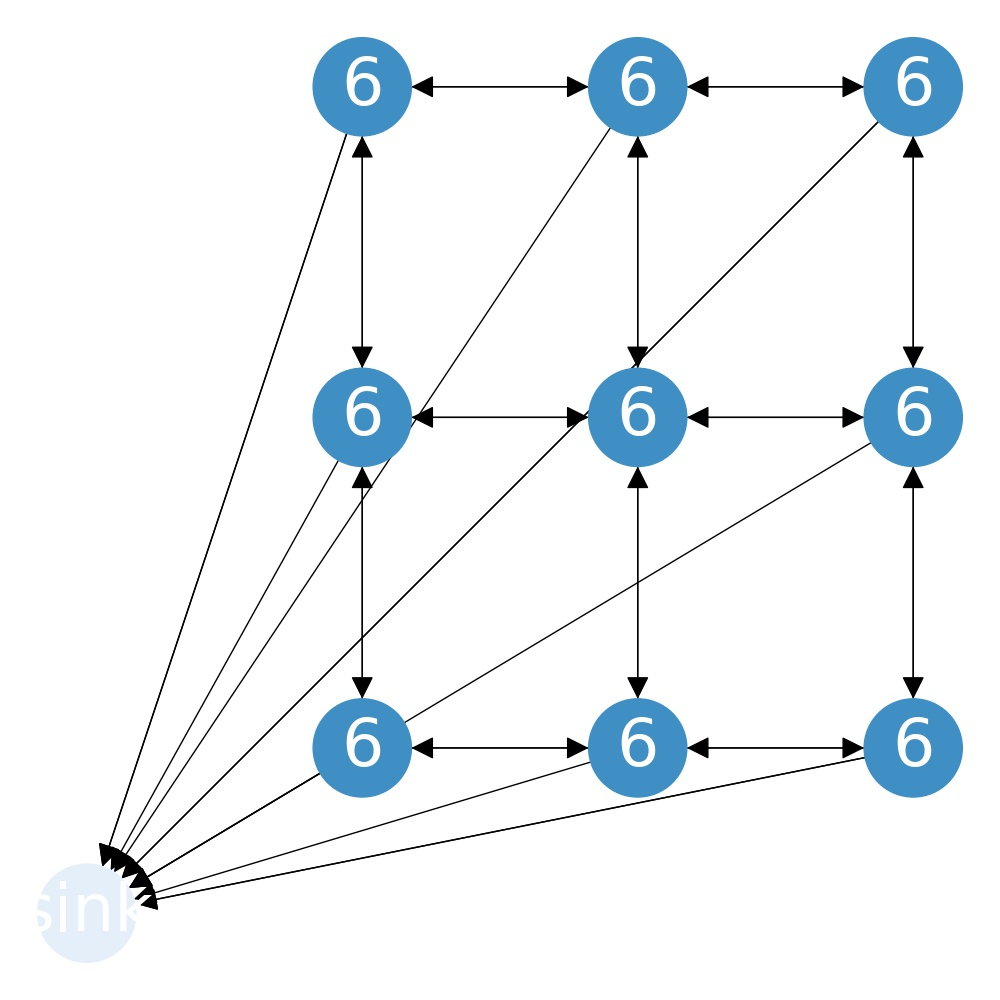
\includegraphics[scale=0.25]{sandpile_0}
      \end{figure}
    \end{frame}
    

    \begin{frame}
      \begin{figure}[h!]
        \centering
          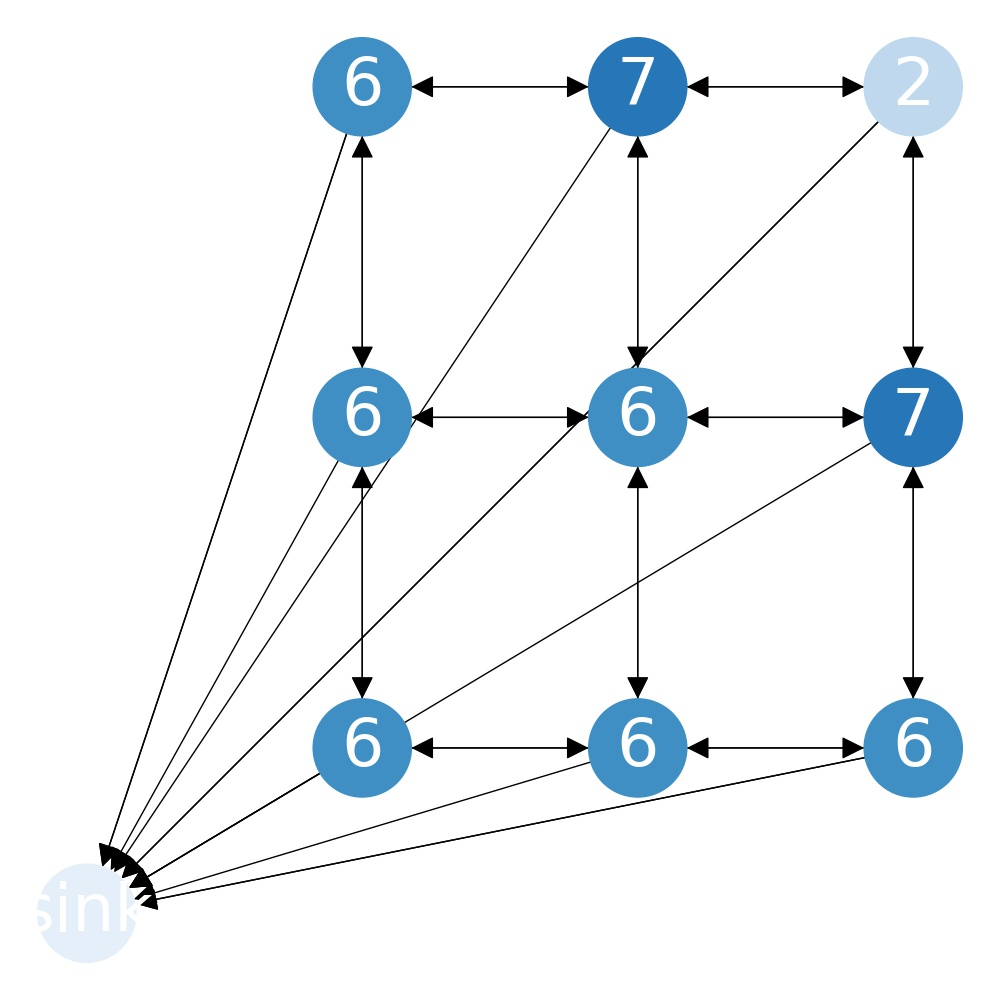
\includegraphics[scale=0.25]{sandpile_-1}
      \end{figure}
    \end{frame}
    

    \begin{frame}
      \begin{figure}[h!]
        \centering
          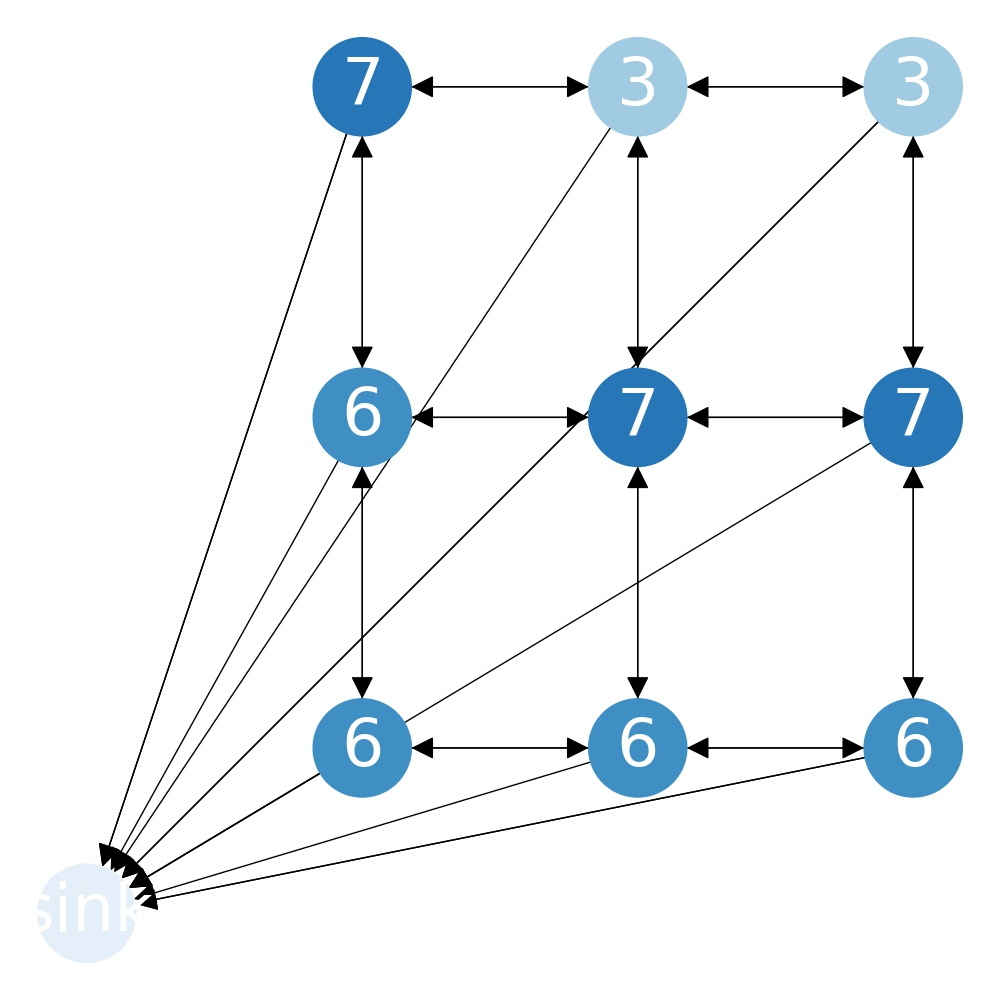
\includegraphics[scale=0.25]{sandpile_-2}
      \end{figure}
    \end{frame}
    

    \begin{frame}
      \begin{figure}[h!]
        \centering
          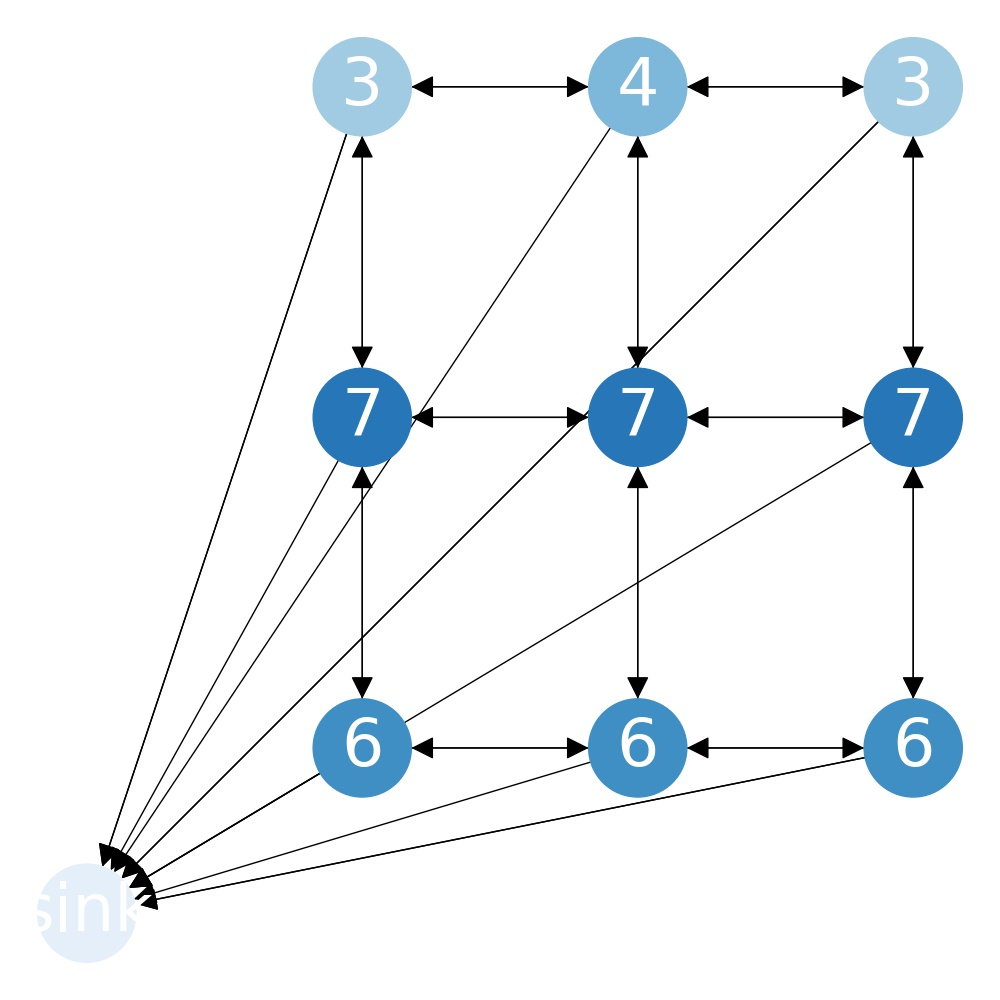
\includegraphics[scale=0.25]{sandpile_-3}
      \end{figure}
    \end{frame}
    

    \begin{frame}
      \begin{figure}[h!]
        \centering
          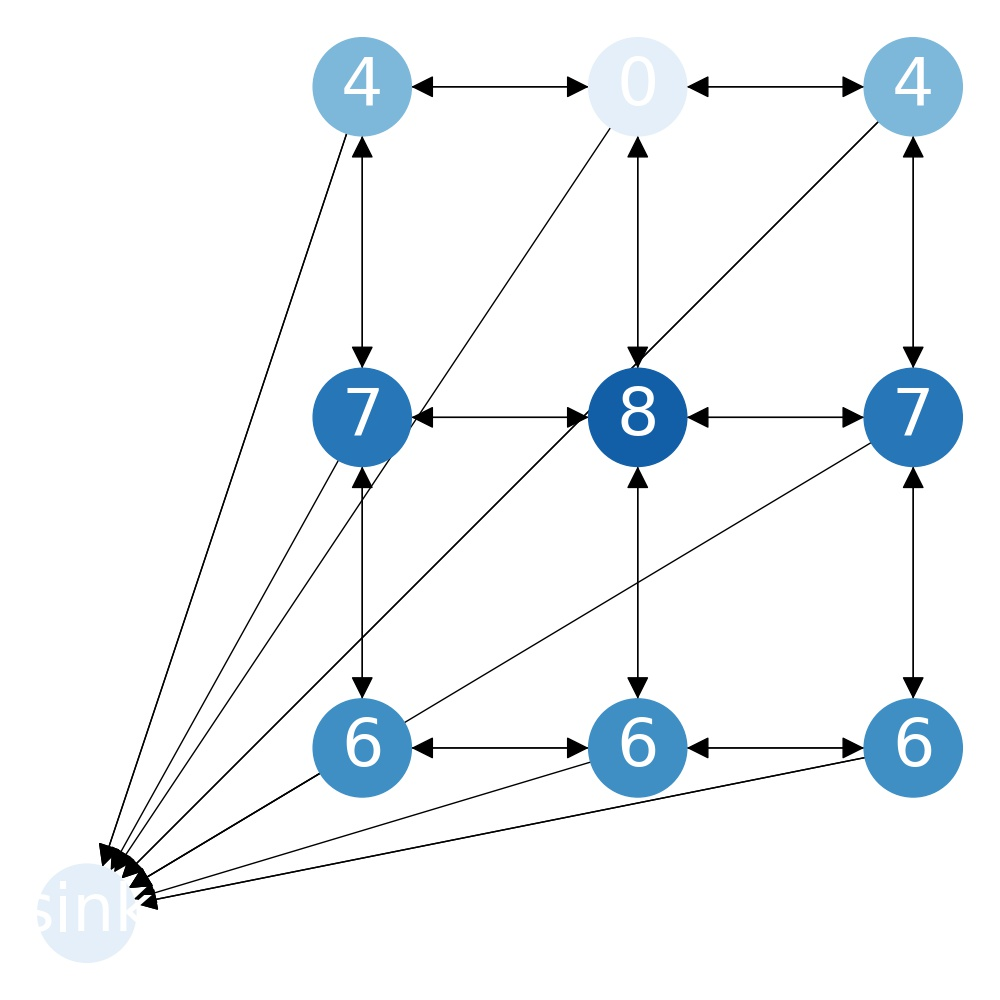
\includegraphics[scale=0.25]{sandpile_-4}
      \end{figure}
    \end{frame}
    

    \begin{frame}
      \begin{figure}[h!]
        \centering
          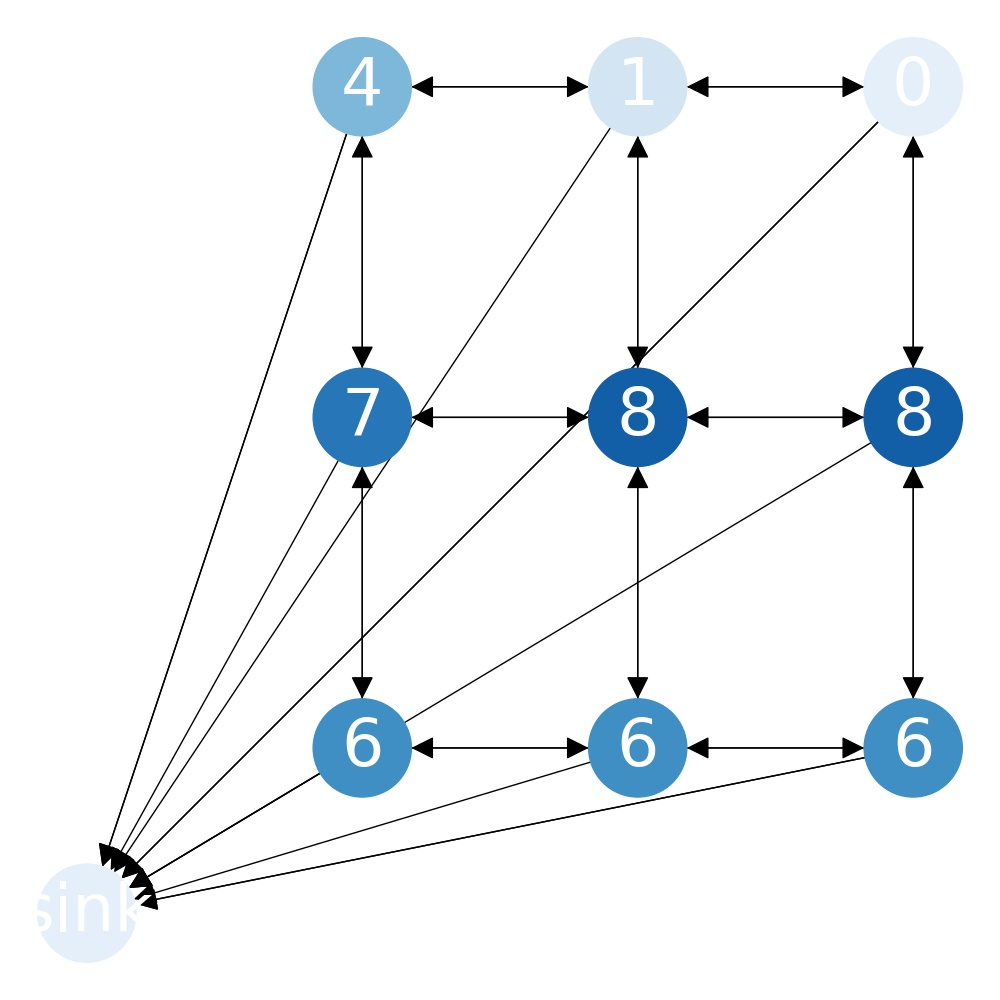
\includegraphics[scale=0.25]{sandpile_-5}
      \end{figure}
    \end{frame}
    

    \begin{frame}
      \begin{figure}[h!]
        \centering
          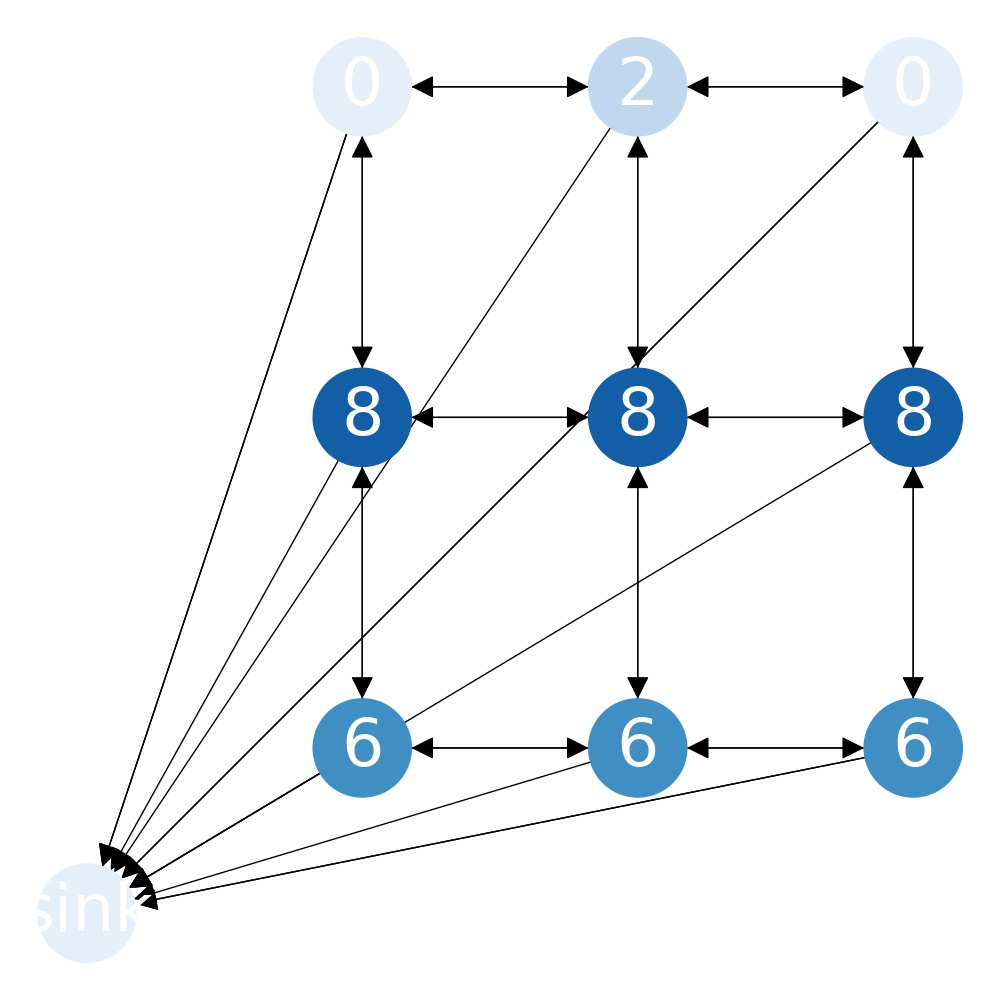
\includegraphics[scale=0.25]{sandpile_-6}
      \end{figure}
    \end{frame}
    

    \begin{frame}
      \begin{figure}[h!]
        \centering
          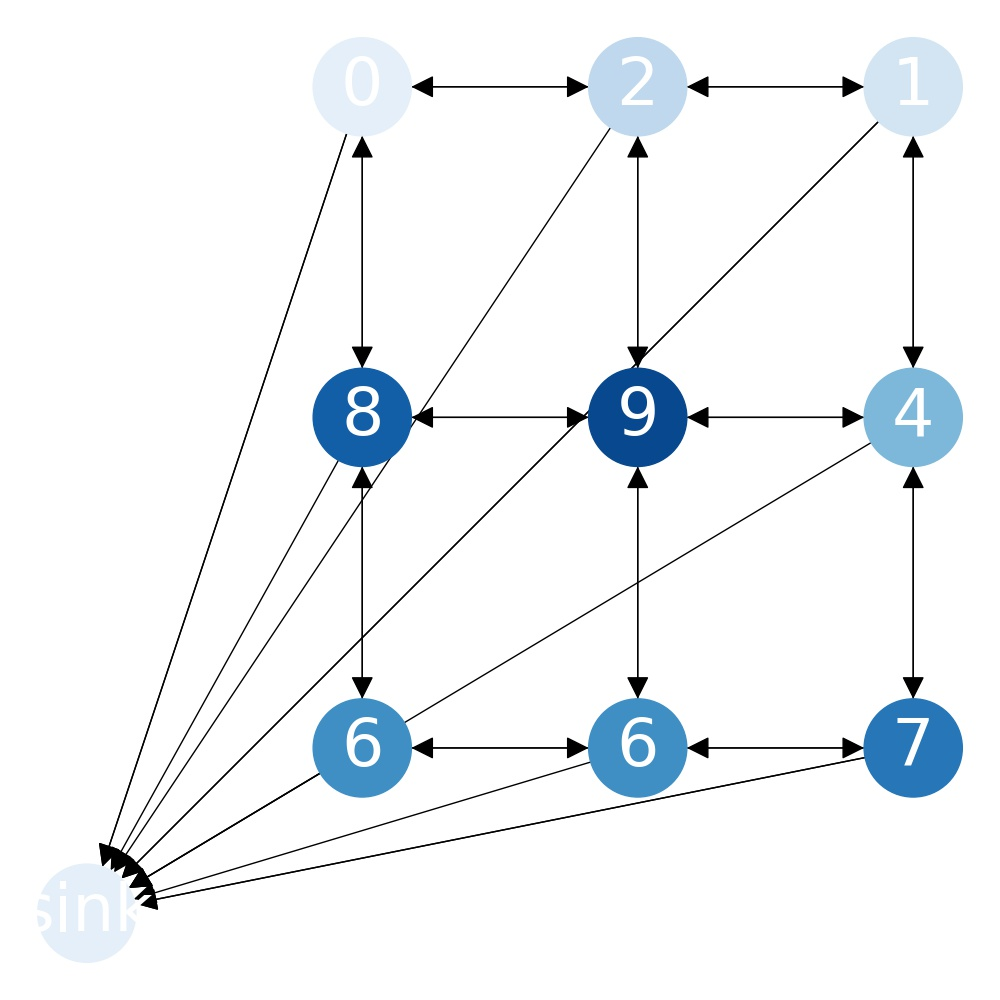
\includegraphics[scale=0.25]{sandpile_-7}
      \end{figure}
    \end{frame}
    

    \begin{frame}
      \begin{figure}[h!]
        \centering
          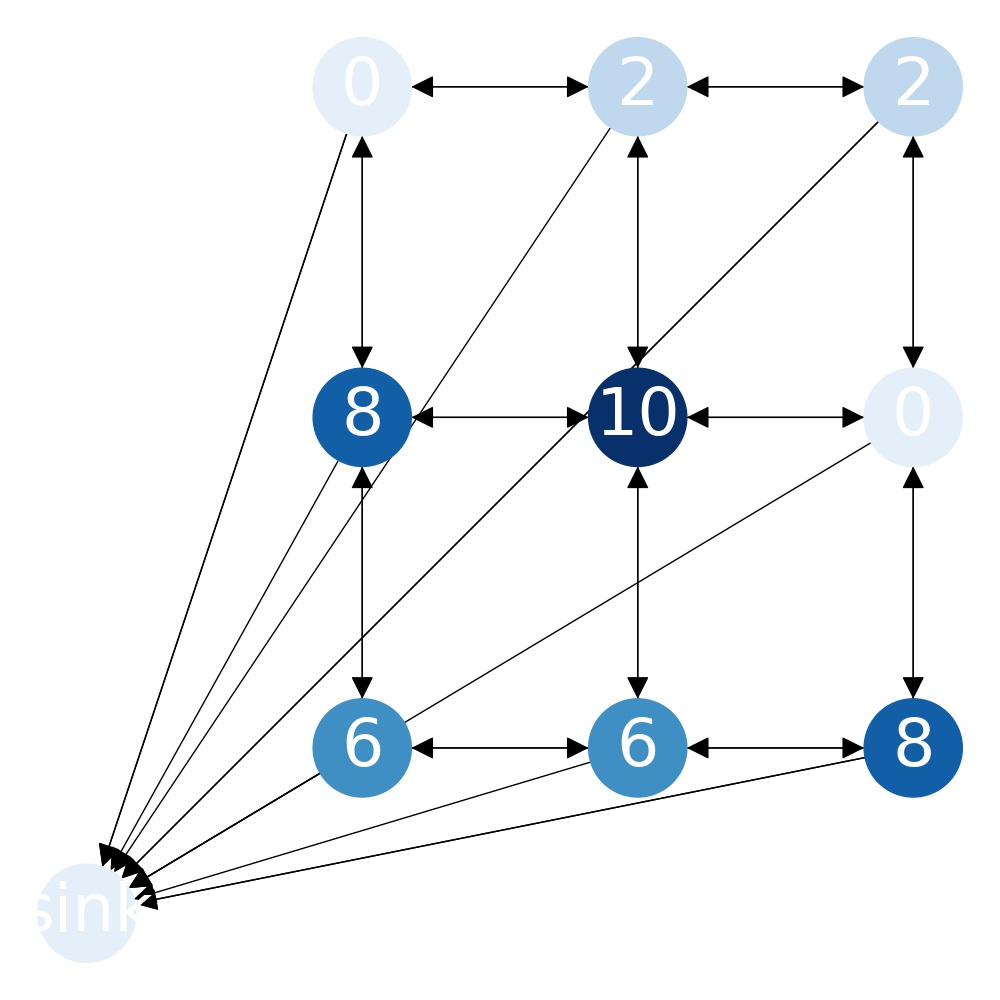
\includegraphics[scale=0.25]{sandpile_-8}
      \end{figure}
    \end{frame}
    

    \begin{frame}
      \begin{figure}[h!]
        \centering
          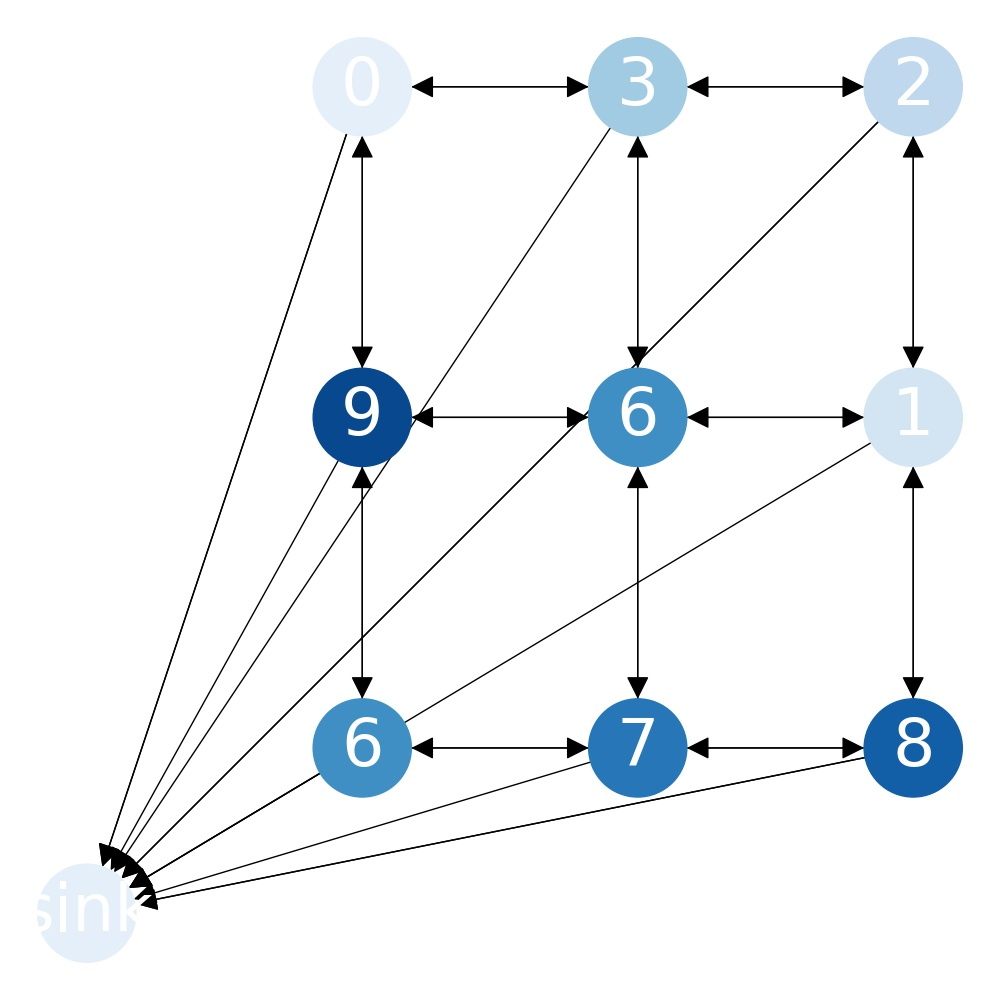
\includegraphics[scale=0.25]{sandpile_-9}
      \end{figure}
    \end{frame}
    

    \begin{frame}
      \begin{figure}[h!]
        \centering
          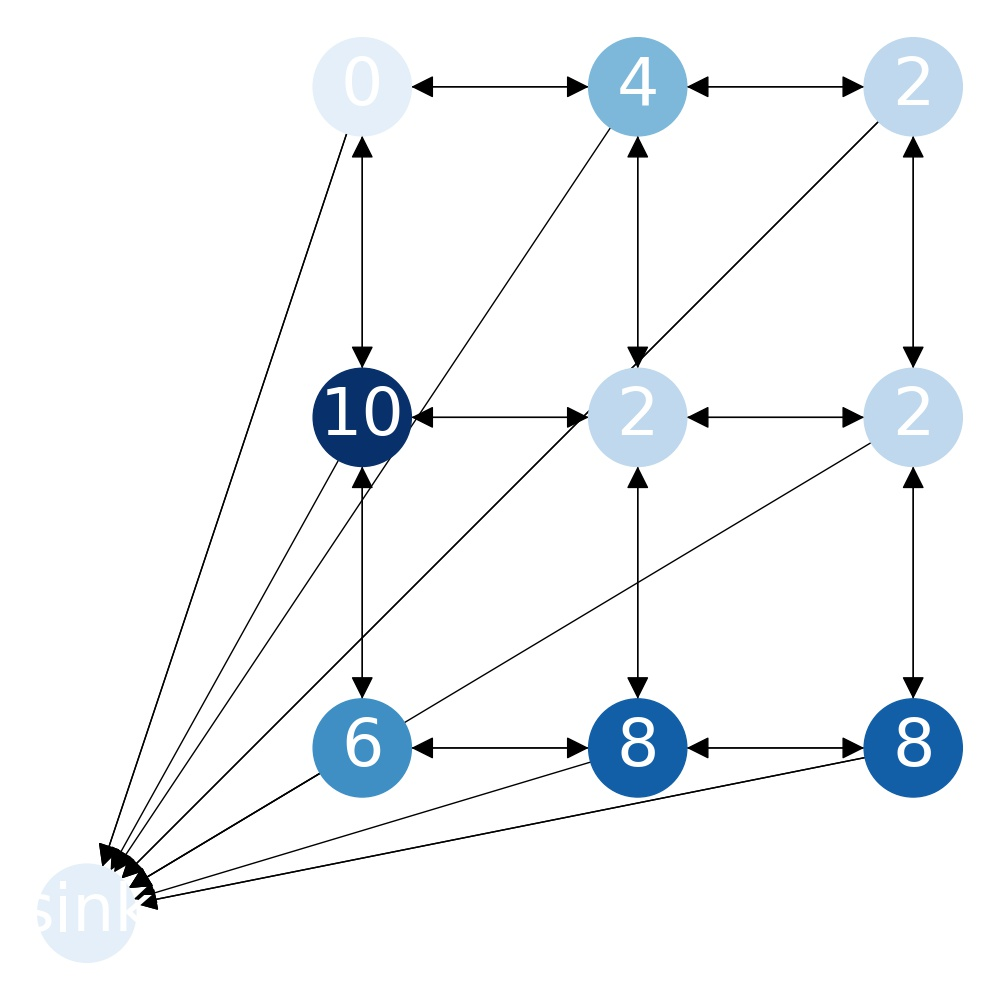
\includegraphics[scale=0.25]{sandpile_-10}
      \end{figure}
    \end{frame}
    

    \begin{frame}
      \begin{figure}[h!]
        \centering
          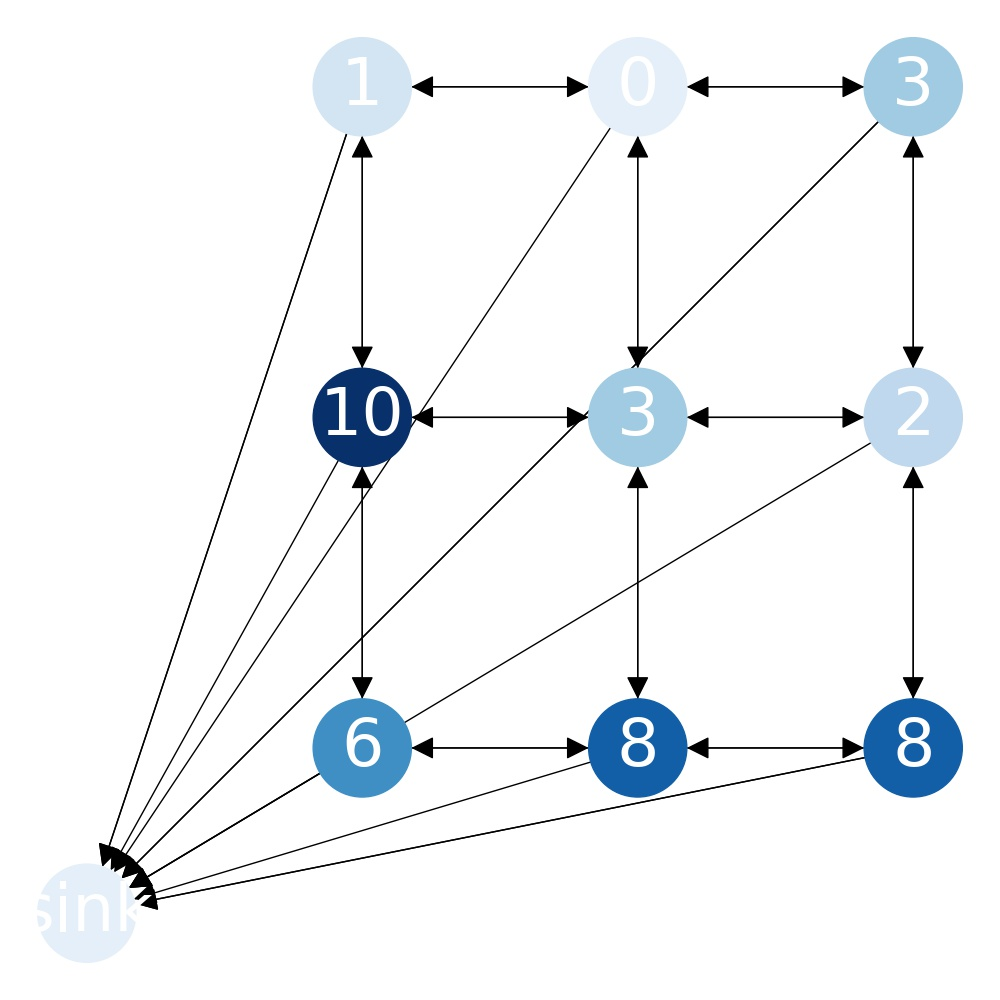
\includegraphics[scale=0.25]{sandpile_-11}
      \end{figure}
    \end{frame}
    

    \begin{frame}
      \begin{figure}[h!]
        \centering
          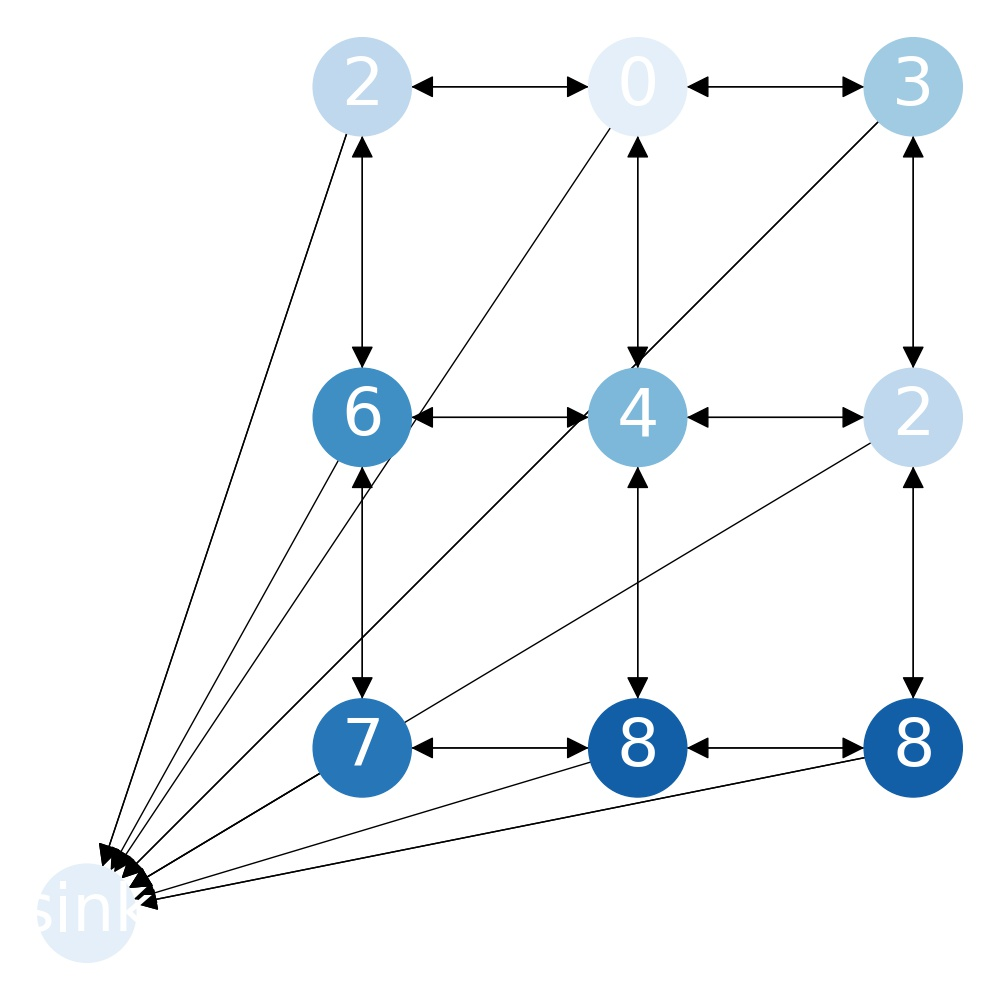
\includegraphics[scale=0.25]{sandpile_-12}
      \end{figure}
    \end{frame}
    

    \begin{frame}
      \begin{figure}[h!]
        \centering
          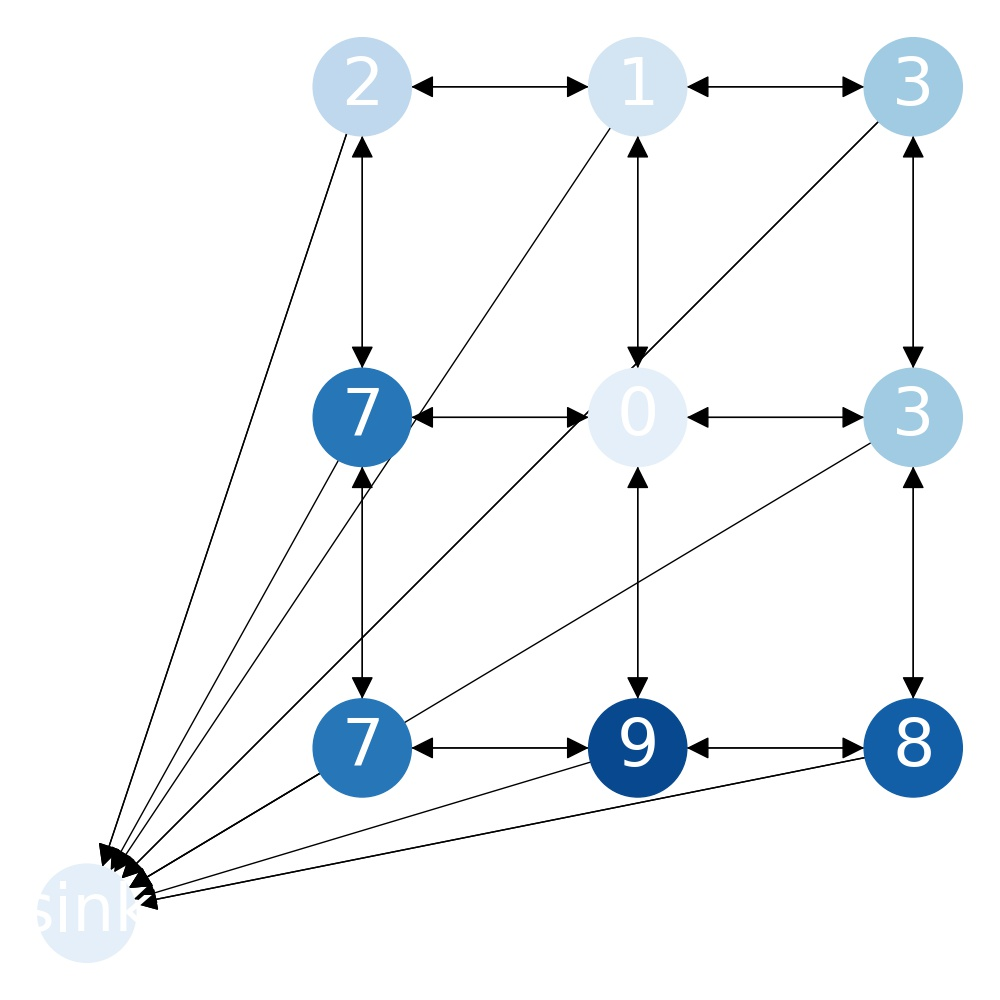
\includegraphics[scale=0.25]{sandpile_-13}
      \end{figure}
    \end{frame}
    

    \begin{frame}
      \begin{figure}[h!]
        \centering
          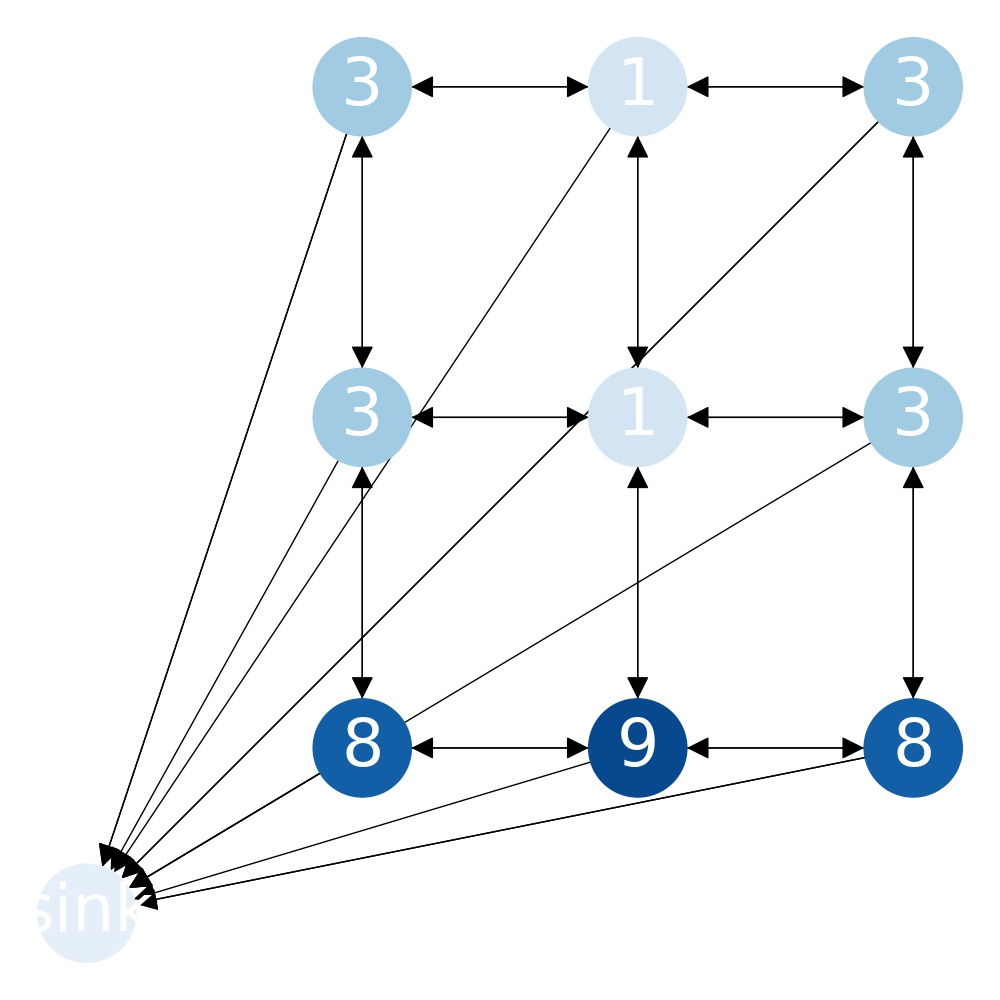
\includegraphics[scale=0.25]{sandpile_-14}
      \end{figure}
    \end{frame}
    

    \begin{frame}
      \begin{figure}[h!]
        \centering
          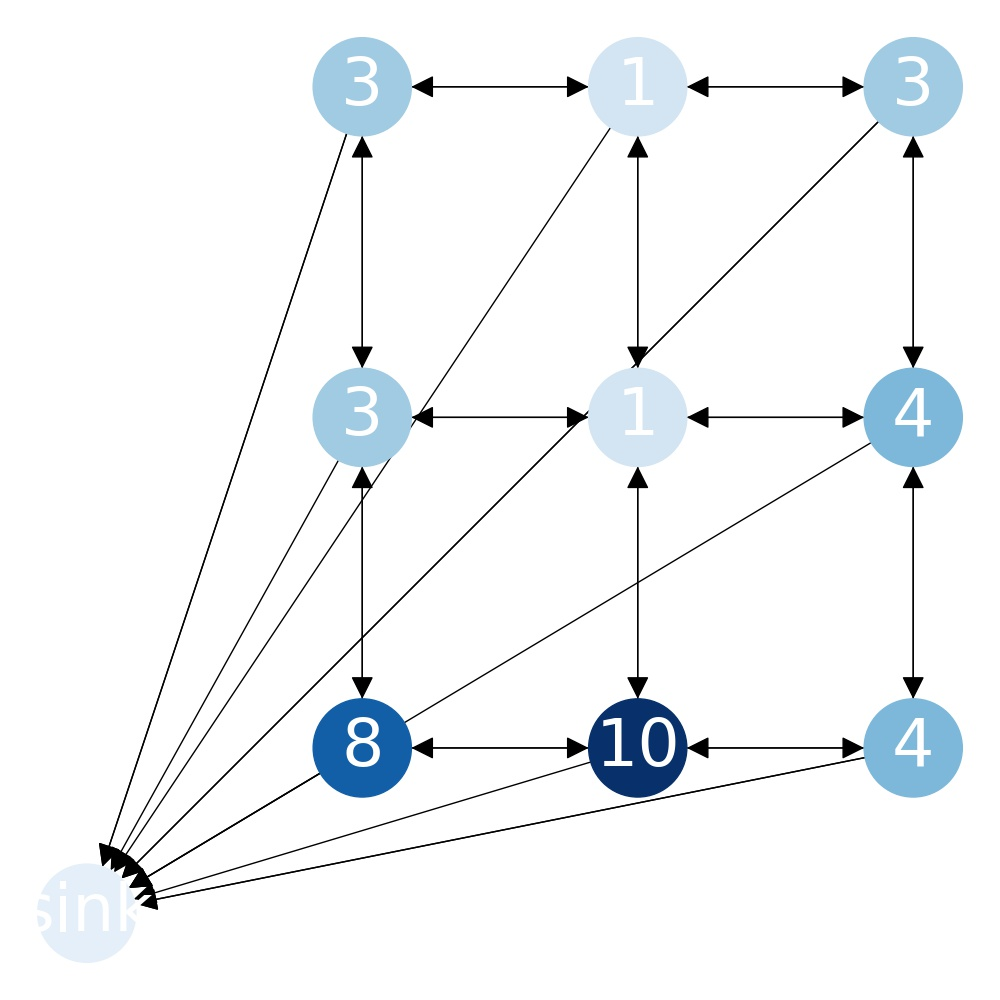
\includegraphics[scale=0.25]{sandpile_-15}
      \end{figure}
    \end{frame}
    

    \begin{frame}
      \begin{figure}[h!]
        \centering
          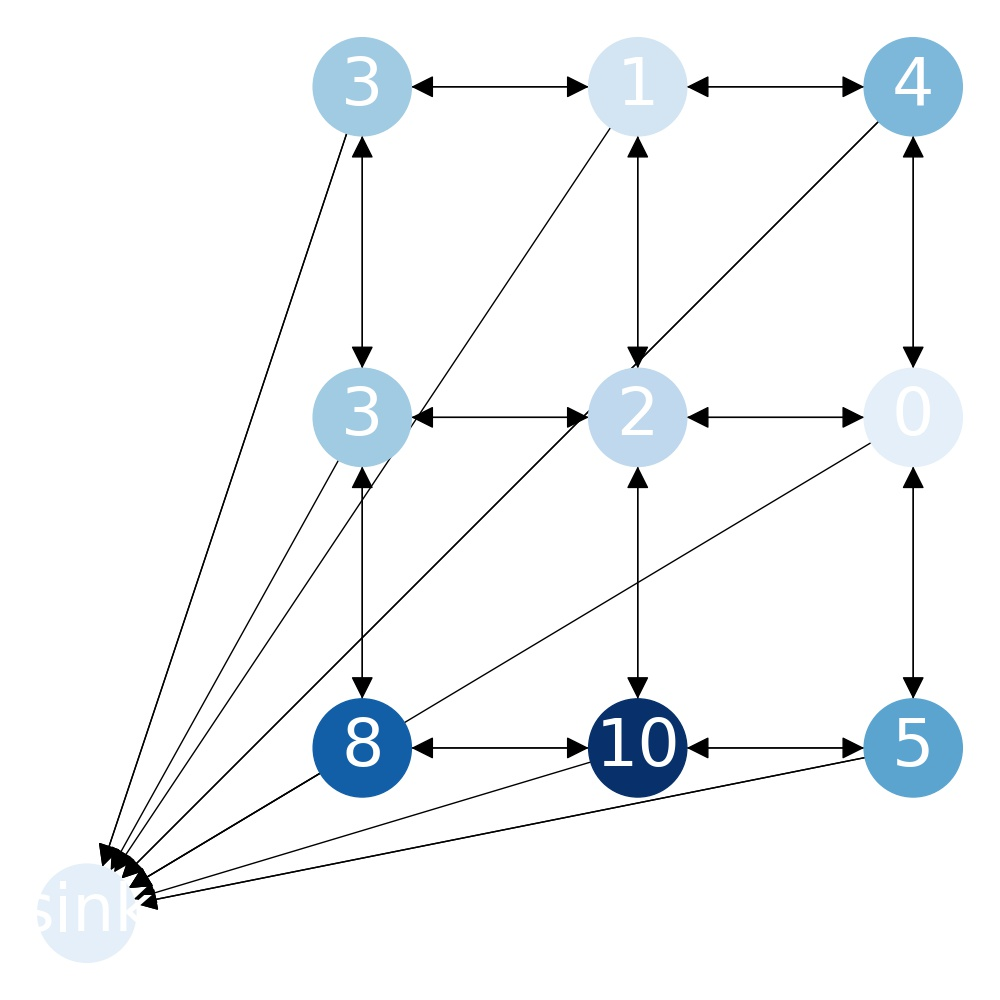
\includegraphics[scale=0.25]{sandpile_-16}
      \end{figure}
    \end{frame}
    

    \begin{frame}
      \begin{figure}[h!]
        \centering
          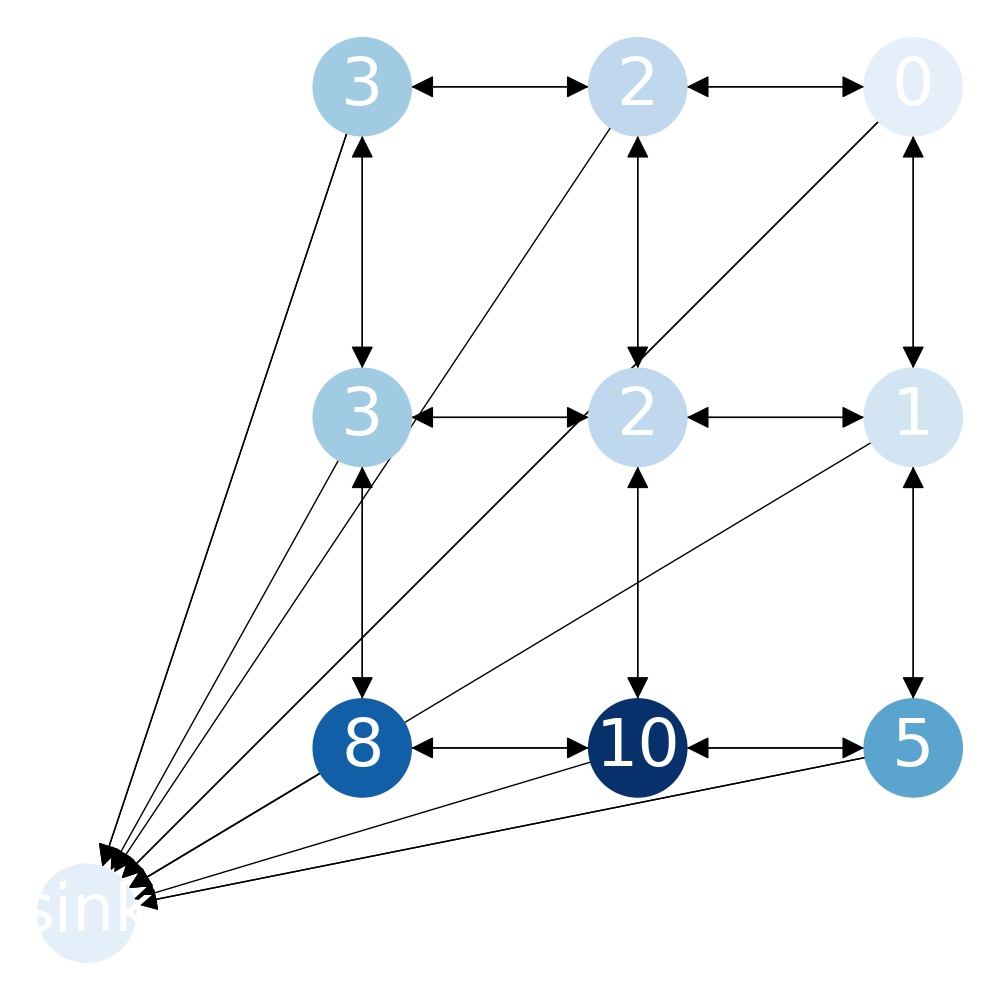
\includegraphics[scale=0.25]{sandpile_-17}
      \end{figure}
    \end{frame}
    

    \begin{frame}
      \begin{figure}[h!]
        \centering
          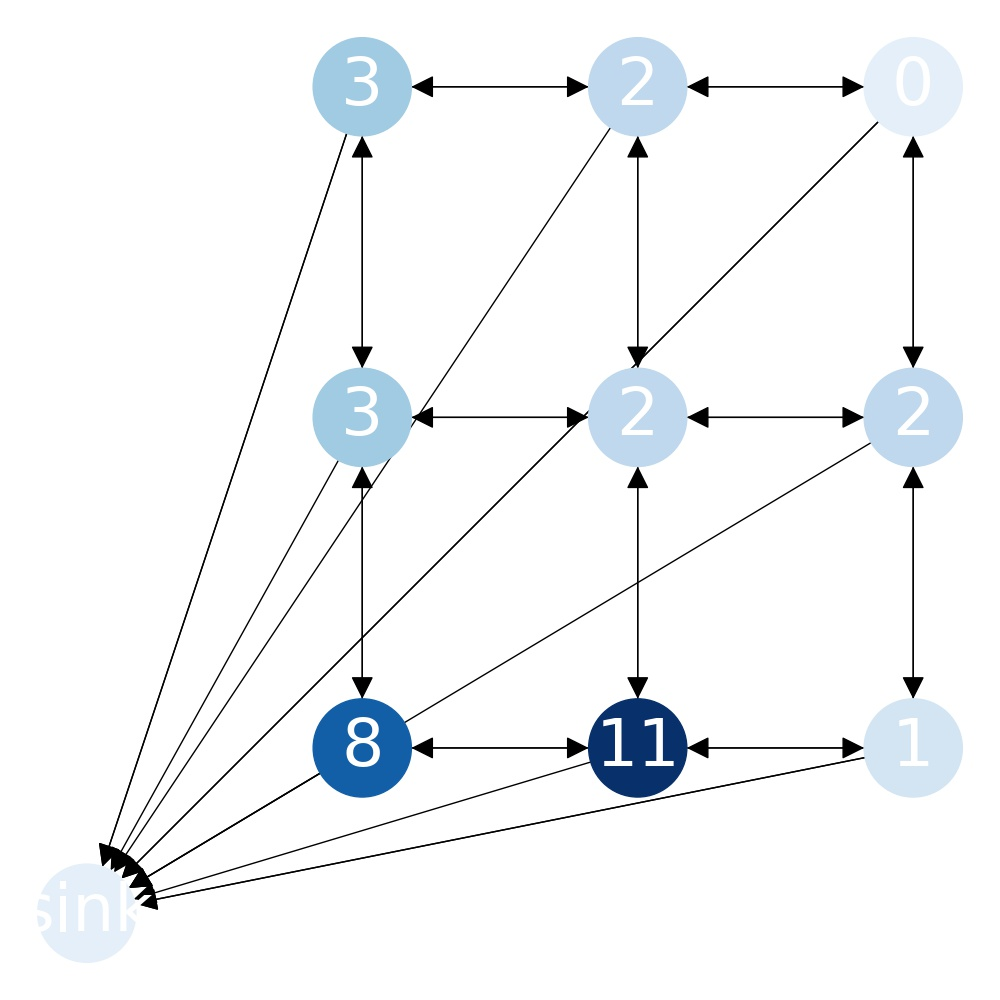
\includegraphics[scale=0.25]{sandpile_-18}
      \end{figure}
    \end{frame}
    

    \begin{frame}
      \begin{figure}[h!]
        \centering
          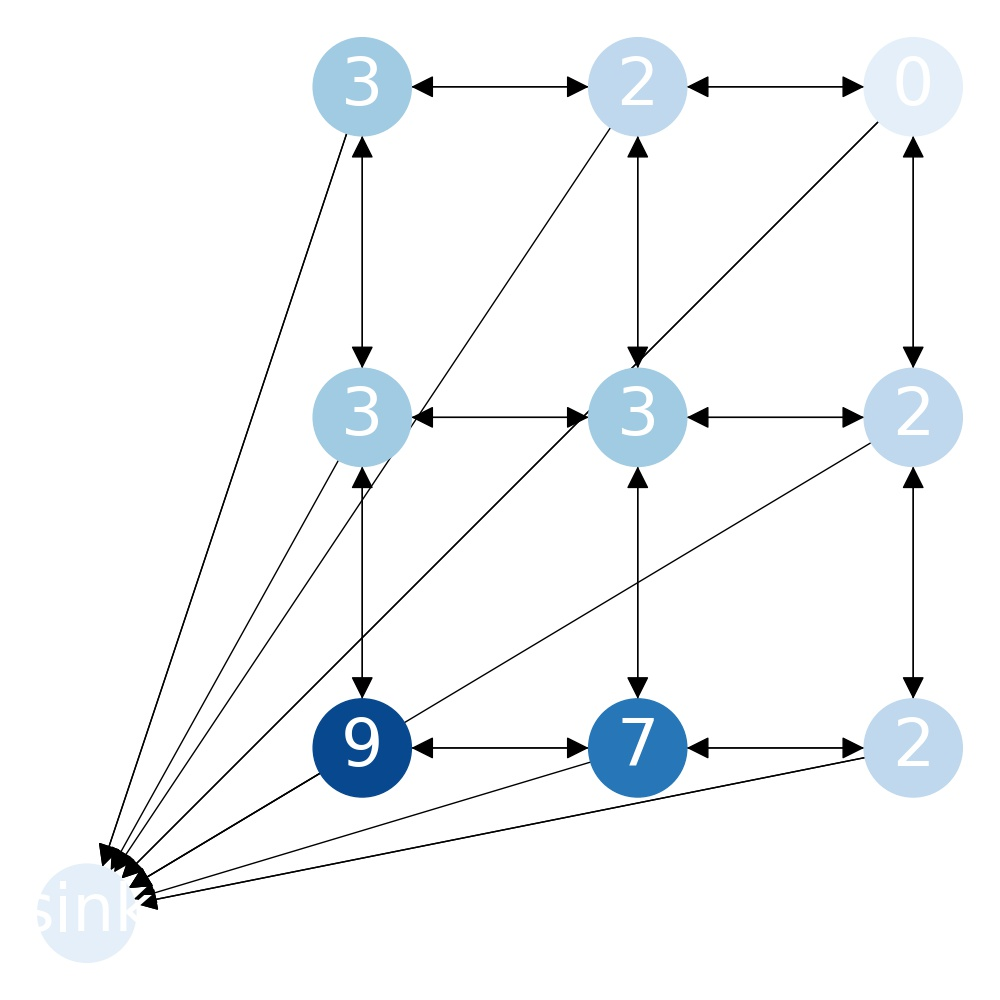
\includegraphics[scale=0.25]{sandpile_-19}
      \end{figure}
    \end{frame}
    

    \begin{frame}
      \begin{figure}[h!]
        \centering
          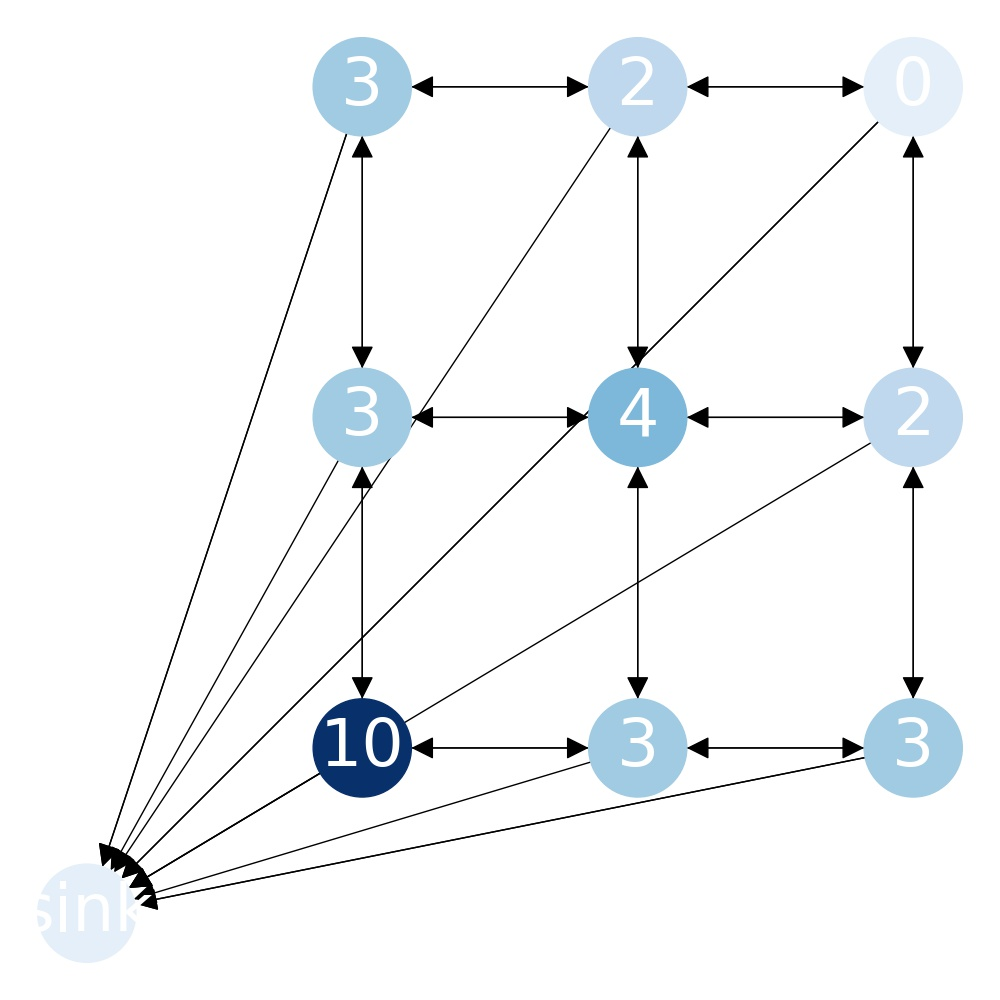
\includegraphics[scale=0.25]{sandpile_-20}
      \end{figure}
    \end{frame}
    

    \begin{frame}
      \begin{figure}[h!]
        \centering
          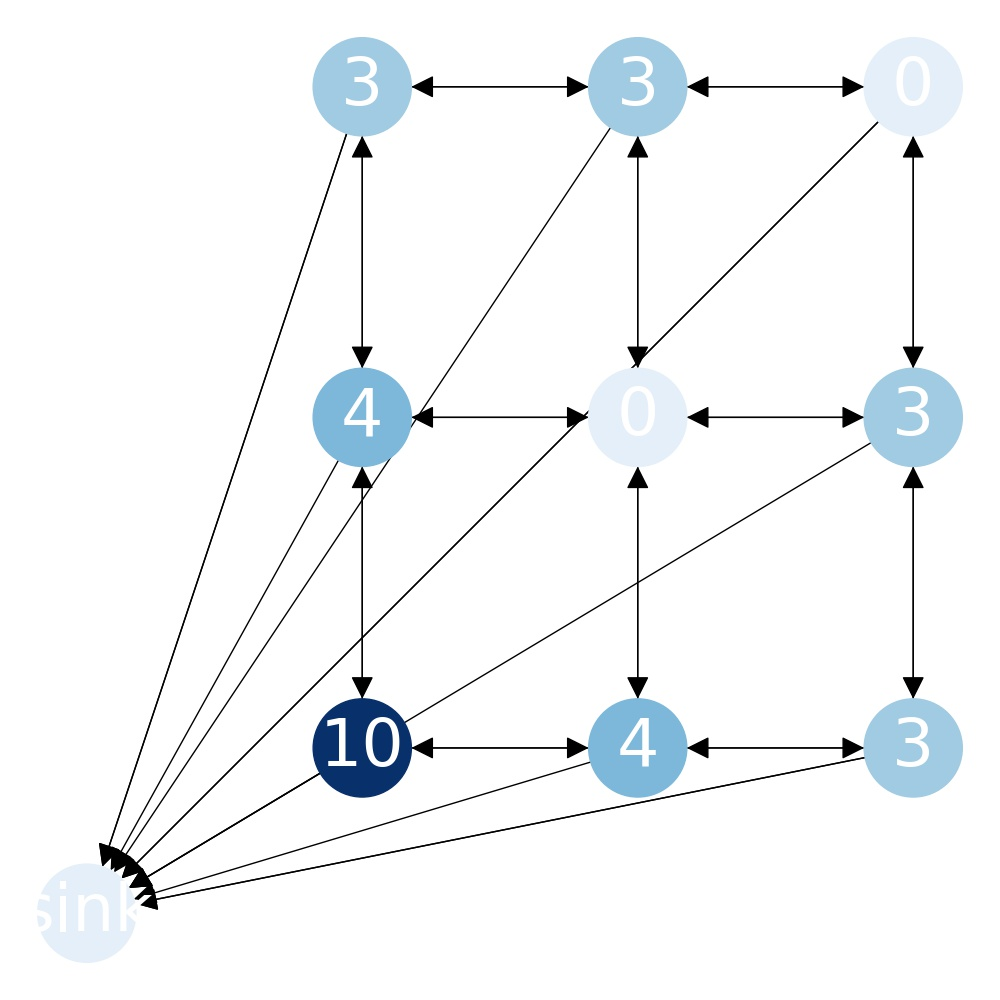
\includegraphics[scale=0.25]{sandpile_-21}
      \end{figure}
    \end{frame}
    

    \begin{frame}
      \begin{figure}[h!]
        \centering
          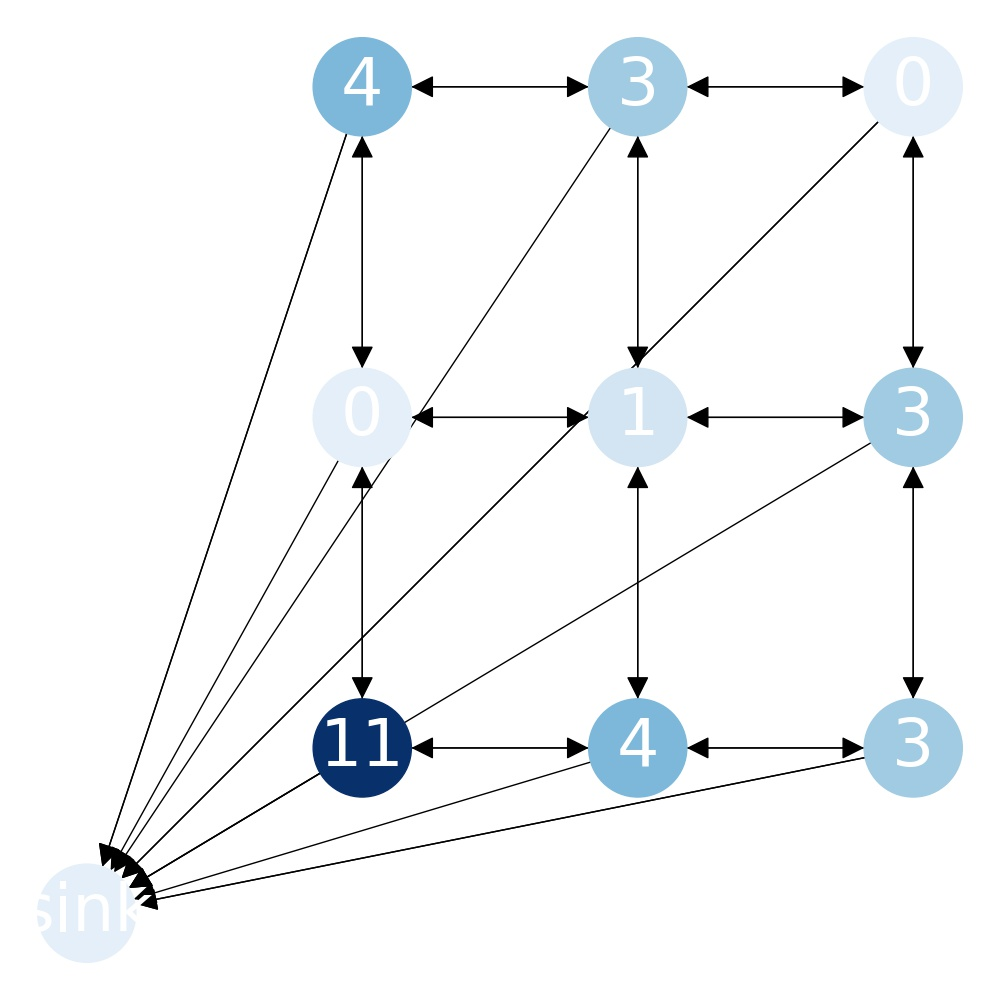
\includegraphics[scale=0.25]{sandpile_-22}
      \end{figure}
    \end{frame}
    

    \begin{frame}
      \begin{figure}[h!]
        \centering
          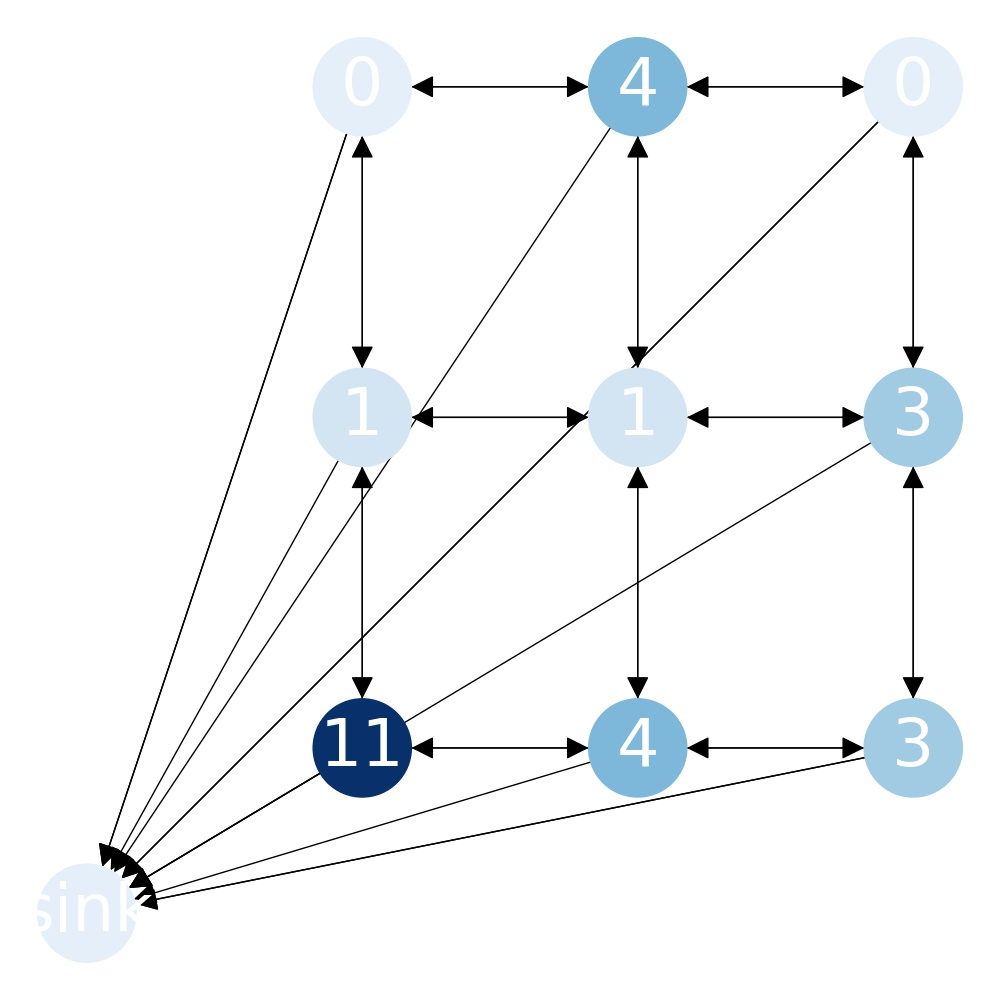
\includegraphics[scale=0.25]{sandpile_-23}
      \end{figure}
    \end{frame}
    

    \begin{frame}
      \begin{figure}[h!]
        \centering
          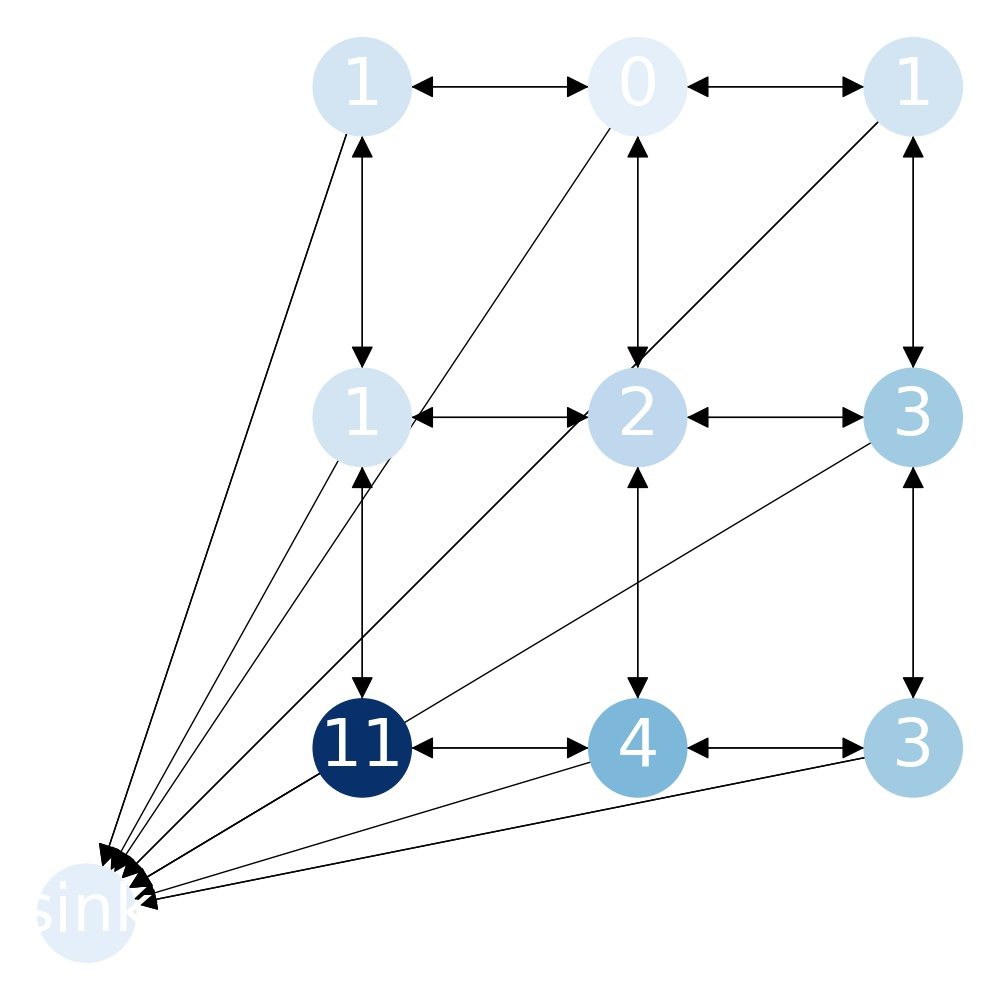
\includegraphics[scale=0.25]{sandpile_-24}
      \end{figure}
    \end{frame}
    

    \begin{frame}
      \begin{figure}[h!]
        \centering
          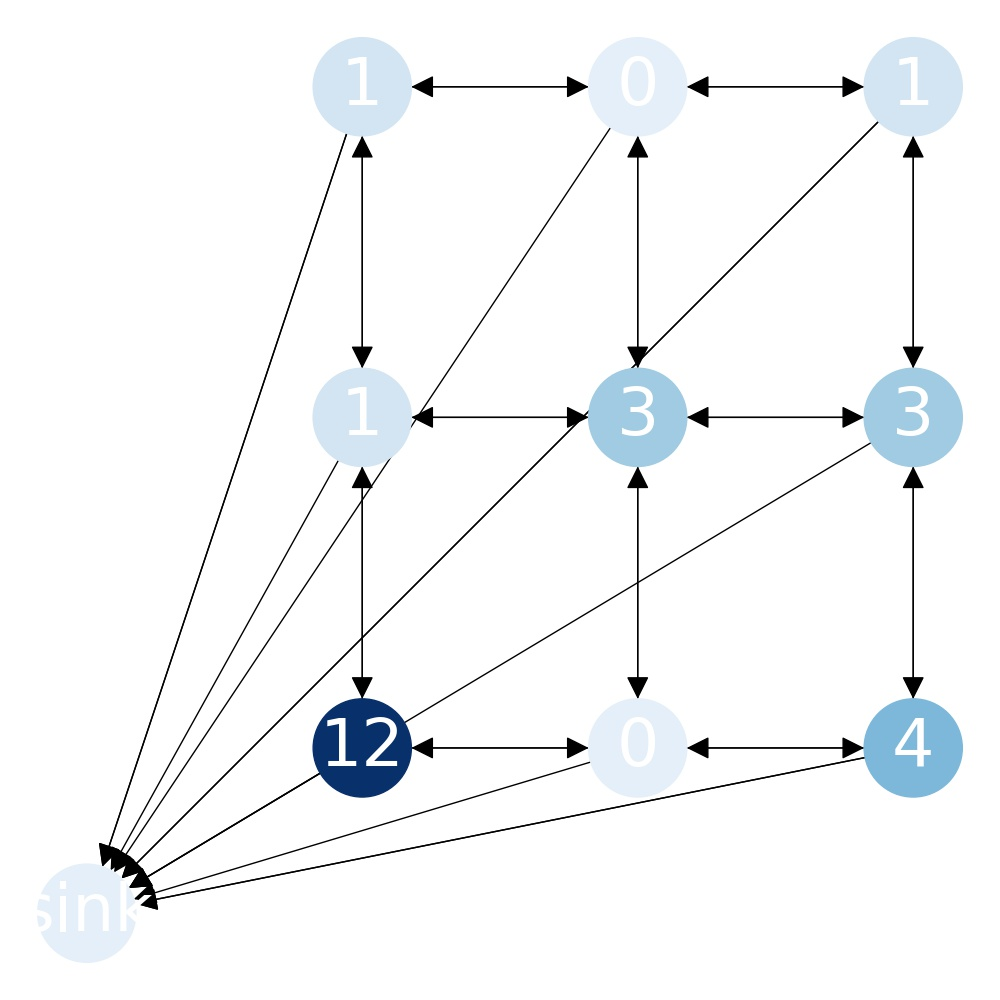
\includegraphics[scale=0.25]{sandpile_-25}
      \end{figure}
    \end{frame}
    

    \begin{frame}
      \begin{figure}[h!]
        \centering
          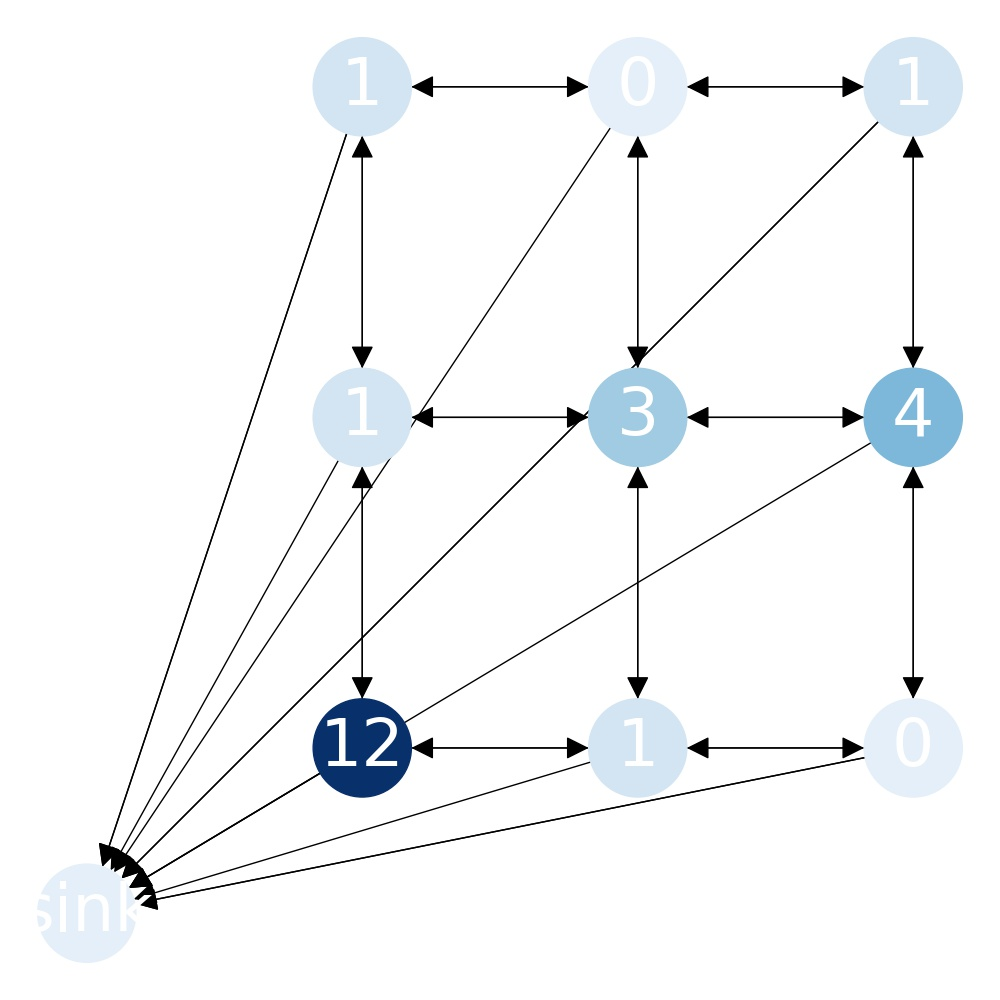
\includegraphics[scale=0.25]{sandpile_-26}
      \end{figure}
    \end{frame}
    

    \begin{frame}
      \begin{figure}[h!]
        \centering
          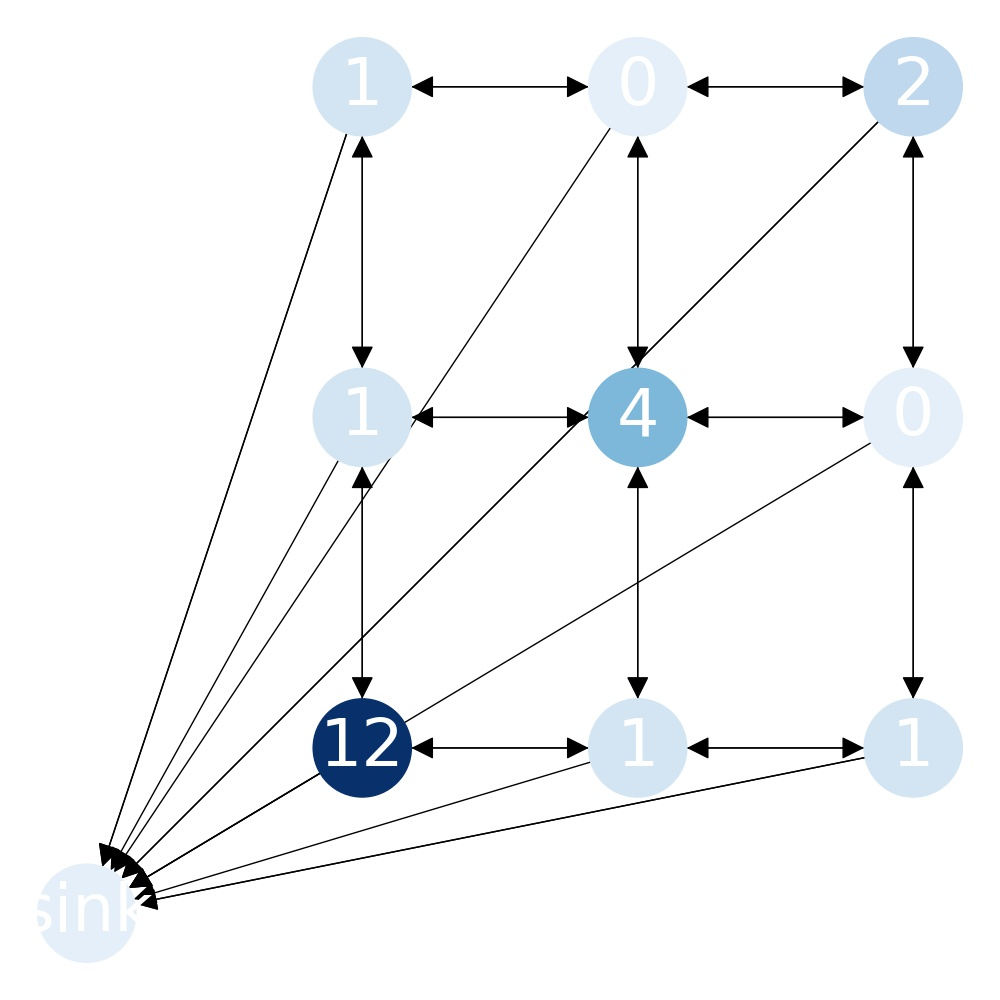
\includegraphics[scale=0.25]{sandpile_-27}
      \end{figure}
    \end{frame}
    

    \begin{frame}
      \begin{figure}[h!]
        \centering
          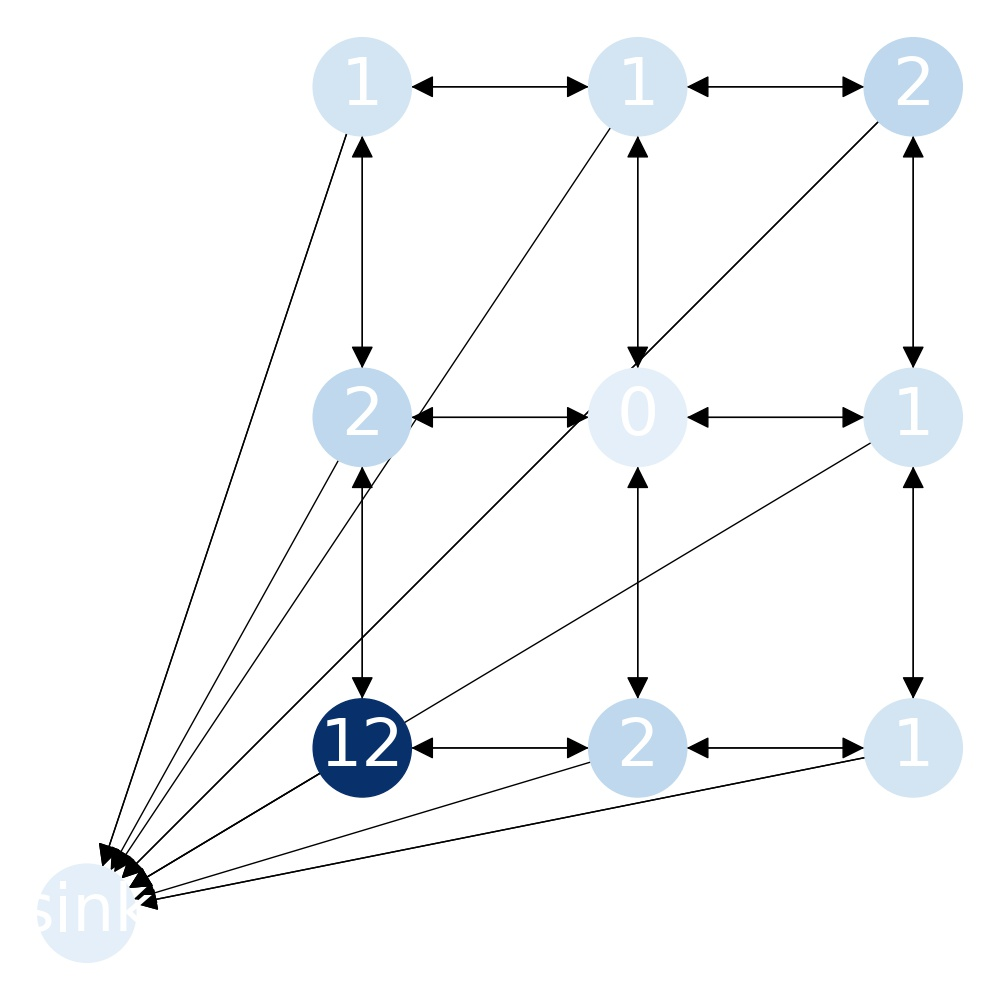
\includegraphics[scale=0.25]{sandpile_-28}
      \end{figure}
    \end{frame}
    

    \begin{frame}
      \begin{figure}[h!]
        \centering
          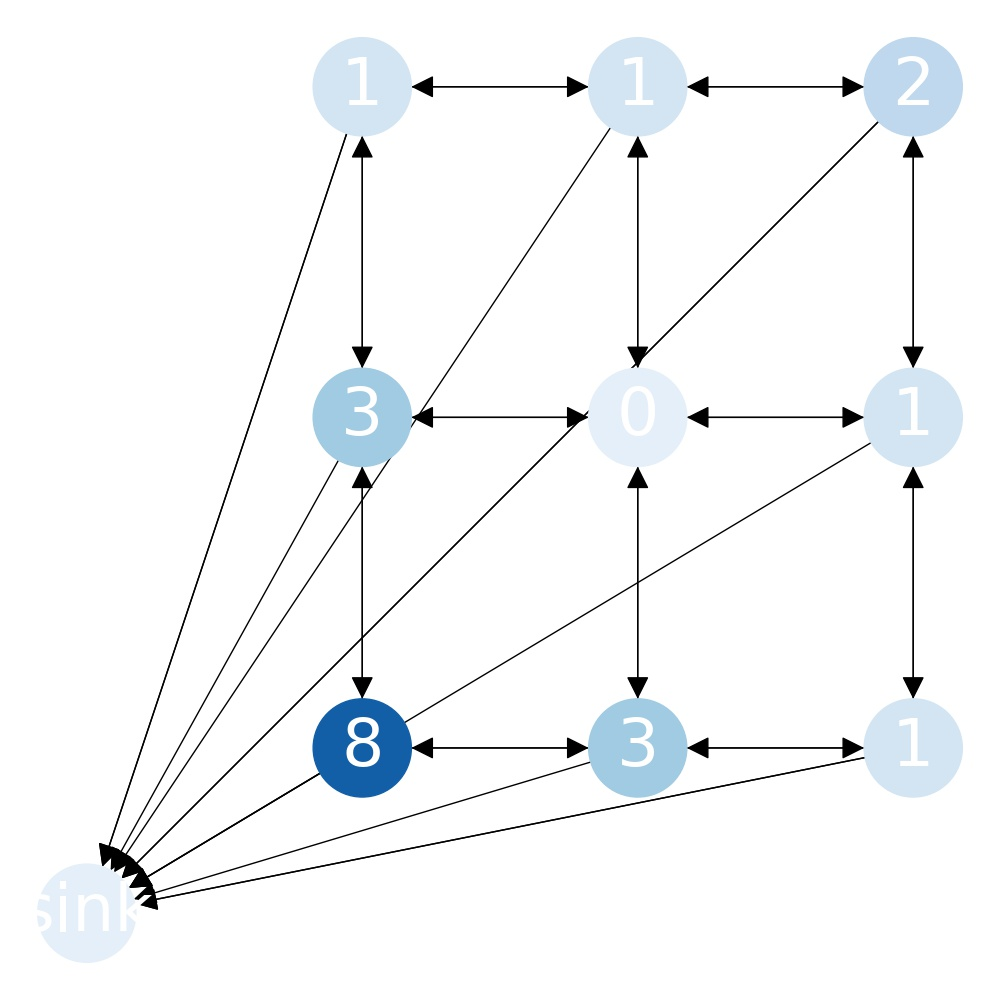
\includegraphics[scale=0.25]{sandpile_-29}
      \end{figure}
    \end{frame}
    

    \begin{frame}
      \begin{figure}[h!]
        \centering
          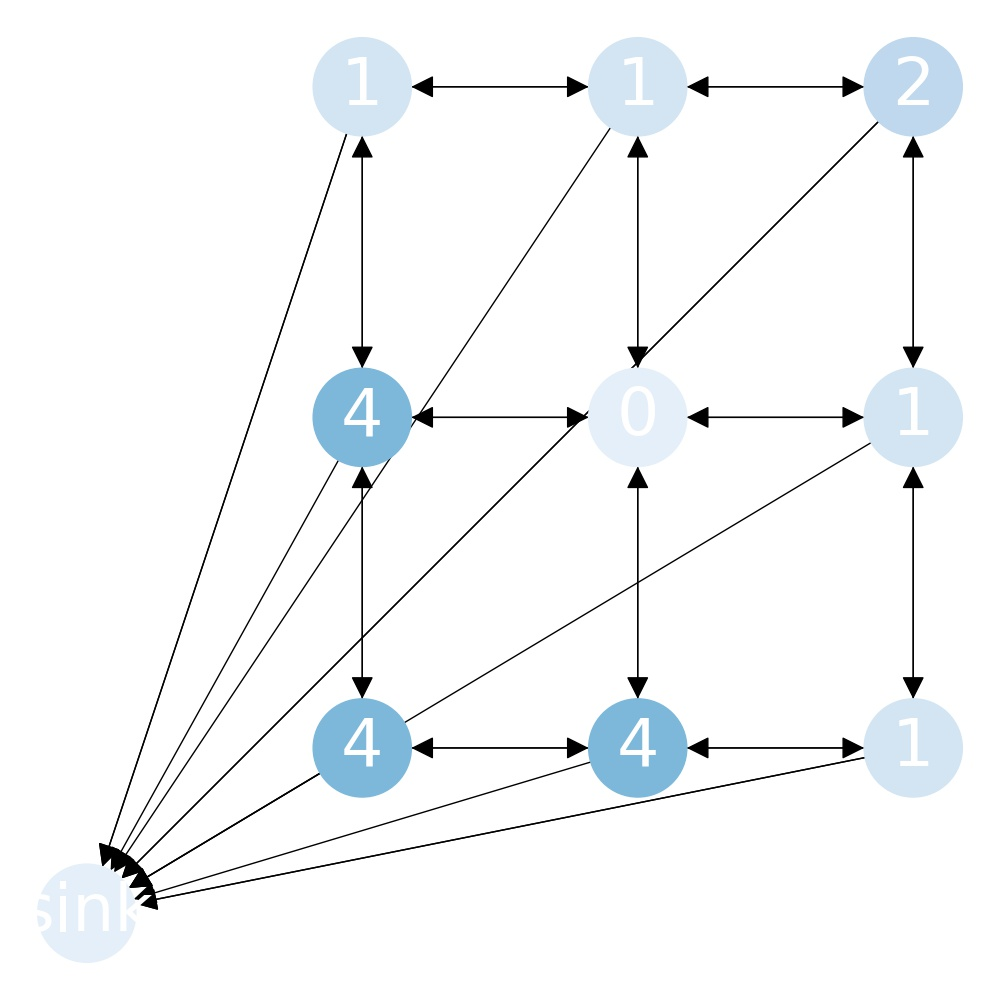
\includegraphics[scale=0.25]{sandpile_-30}
      \end{figure}
    \end{frame}
    

    \begin{frame}
      \begin{figure}[h!]
        \centering
          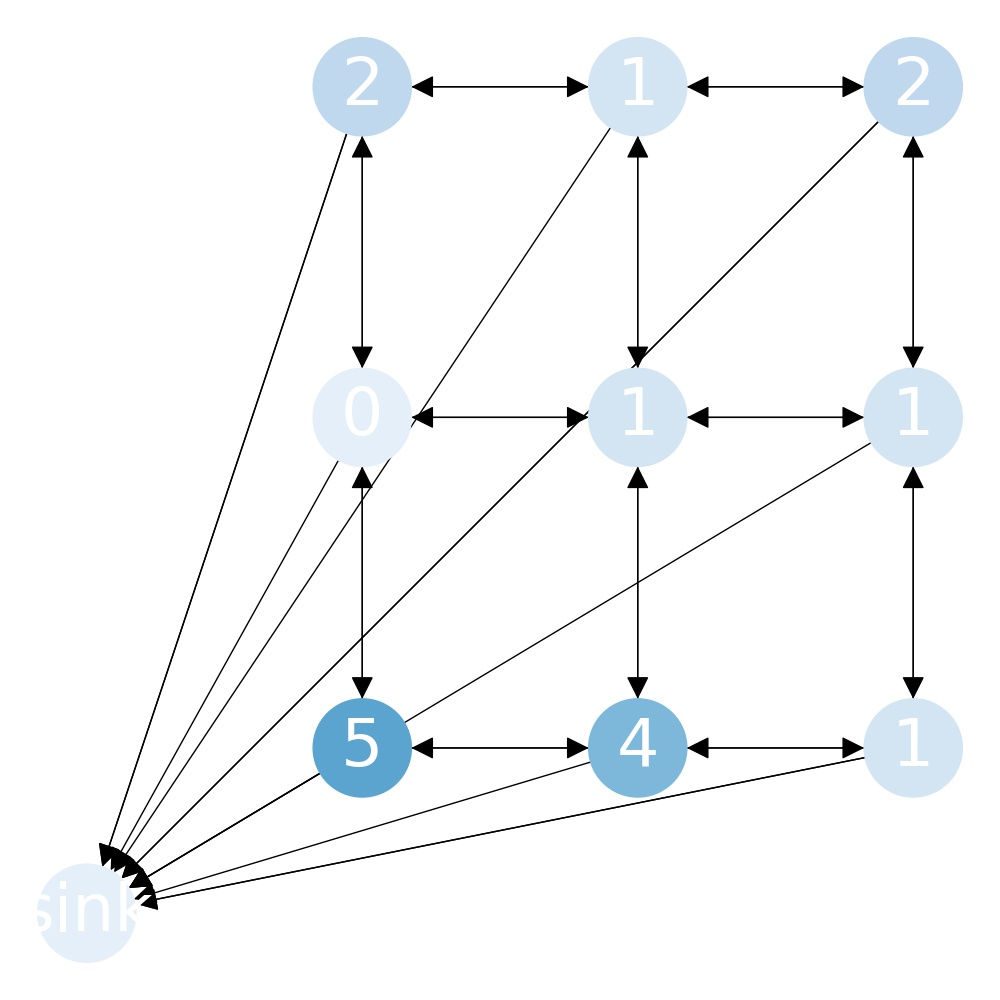
\includegraphics[scale=0.25]{sandpile_-31}
      \end{figure}
    \end{frame}
    

    \begin{frame}
      \begin{figure}[h!]
        \centering
          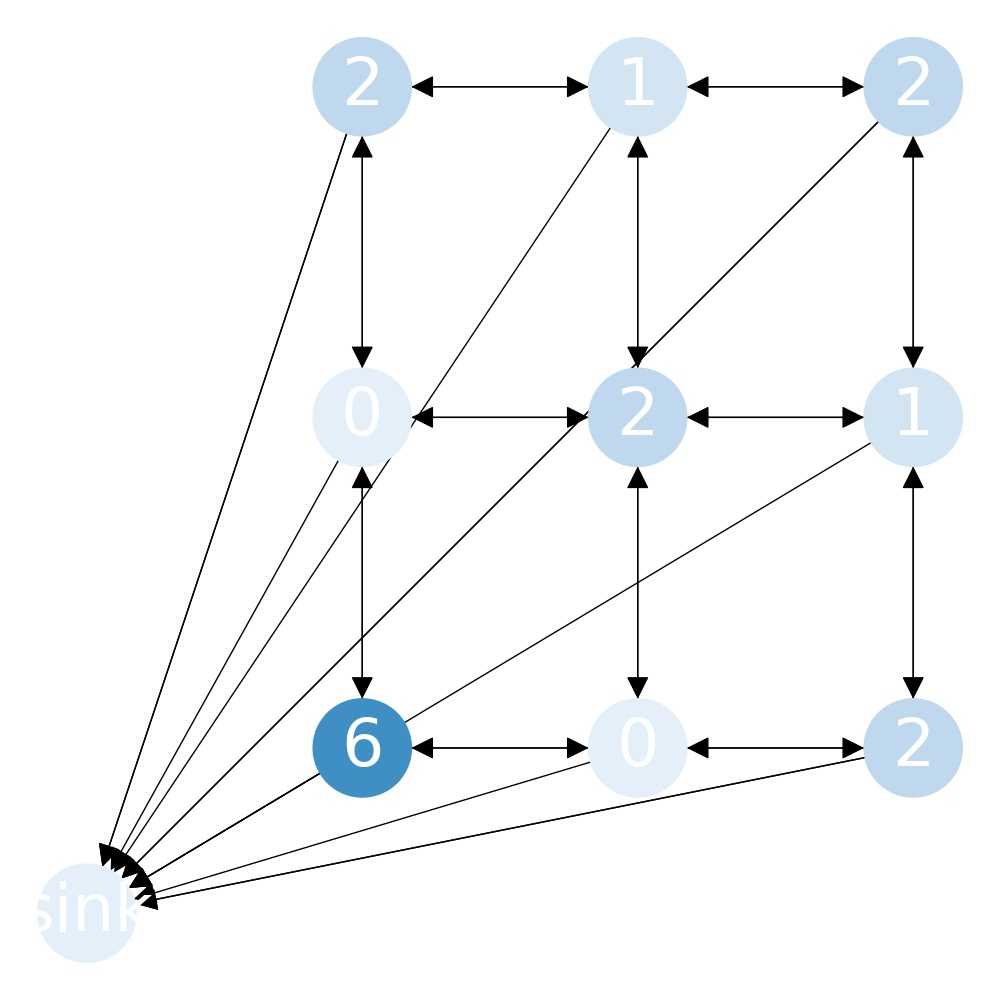
\includegraphics[scale=0.25]{sandpile_-32}
      \end{figure}
    \end{frame}
    

    \begin{frame}
      \begin{figure}[h!]
        \centering
          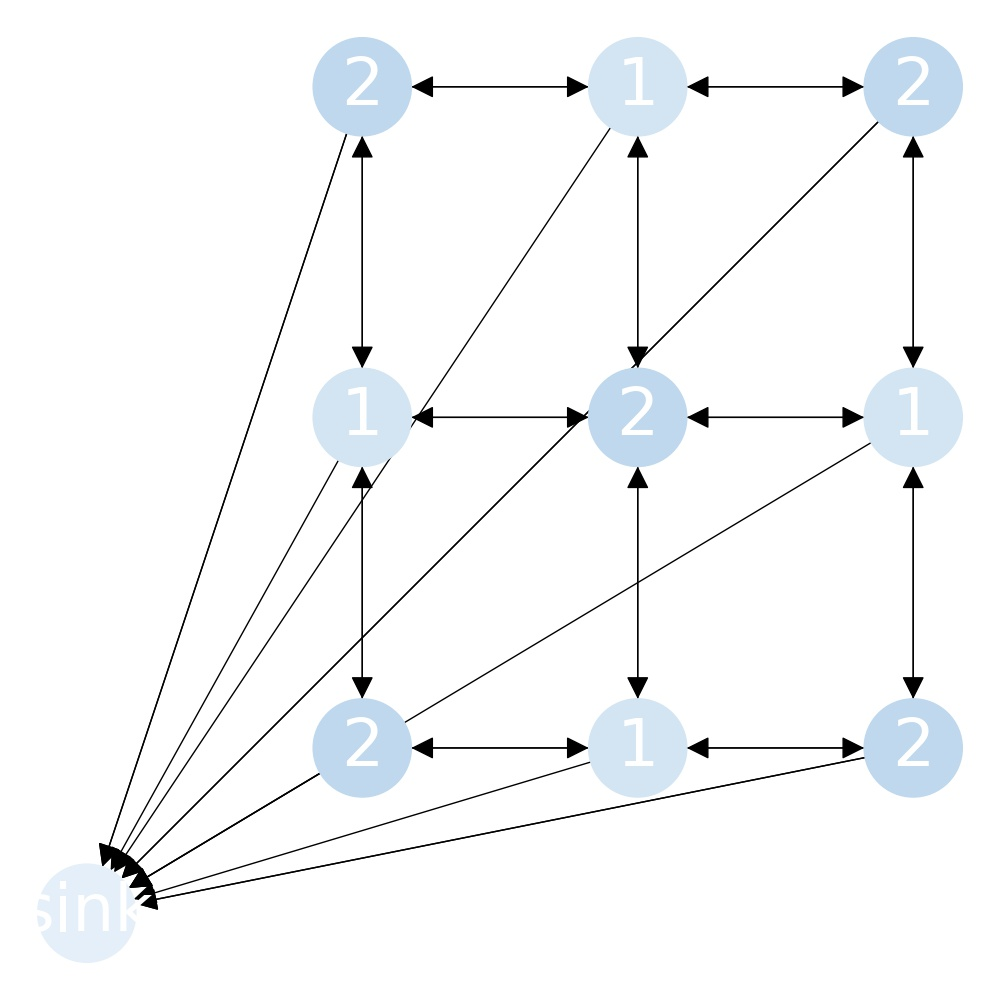
\includegraphics[scale=0.25]{sandpile_-33}
      \end{figure}
    \end{frame}
    

    \end{document}
    